\chapter{Event Categorisation}
\label{chap:event_select}

%\newpage
\section{Overview and Objectives}
Once a set of candidate photons is assembled they are tagged and categorised using extra final-state objects characteristic of particular Higgs production modes.
The objective of this tagging procedure is to enhance overall significance, to construct categories of events with superior mass resolution, and to separate out the Higgs production modes for individual measurement. 


The event categorisation begins with a selection on the photon candidates with $p_{T}^{\gamma1}/m_{\gamma\gamma} > 1/3$, $p_{T}^{\gamma2}/m_{\gamma\gamma} > 1/4$, and $100 < m_{\gamma\gamma} < 180$\,GeV.
The use of mass-scaled $p_{T}$ here and in later machine learning models serves a dual purpose: firstly it avoids distortion of lower values in the $m_{\gamma\gamma}$ spectrum, secondly it avoids introducing mass bias from the simulated data during model trainings. 
There are then further requirements on the photons' supercluster pseudorapidities: both must have $|\eta| < 2.5$ to keep them in the fiducial region of the ECAL, and also must not be in the barrel-endcap transition region $1.44 < |\eta| < 1.57$ to ensure full containment of the electromagnetic showers. 


\subsection{The Diphoton BDT}
Selected diphoton candidates are then evaluated for signal-like kinematics and mass resolution by a BDT, the diphoton BDT, whose output score is used as a discriminating variable by the tags.
The input features of this BDT are the following:
\begin{itemize}[noitemsep]
    \item the mass-scaled transverse momentum $p^{\gamma}_{T}/m_{\gamma\gamma}$ for the leading and subleading photons;
    \item the pseudorapidity $\eta$ for the leading and subleading photons;
    \item the cosine of the azimuthal angle $\Delta\phi$ between the photons;
    \item the score from the photon identification BDT for both photons;
    \item the mass resolution estimate given the assumption that the correct vertex is selected, $\sigma^{RV}_{\gamma\gamma}/m_{\gamma\gamma}$;
    \item the mass resolution estimate given the assumption that the incorrect vertex is selected, $\sigma^{WV}_{\gamma\gamma}/m_{\gamma\gamma}$;
    \item the probability that the correct diphoton vertex has been selected $p^{RV}$,, estimated with the vertex probability BDT.
\end{itemize}

The mass resolution in the right vertex case, $\sigma^{RV}_{\gamma\gamma}/m_{\gamma\gamma}$, is assumed to be completely dominated by the ECAL photon energy resolution; one can therefore neglect vertex uncertainty. The energy resolution for each photon can be approximated by a Gaussian distribution and combined in quadrature to give the following expression for mass resolution,
\begin{equation}
    \sigma^{RV}_{\gamma\gamma} = \frac{1}{2}\sqrt{(\sigma^{E}_{\gamma{1}}/E_{\gamma{1}})^2 + (\sigma^{E}_{\gamma{2}}/E_{\gamma{2}})^2}
\end{equation} 
where $\sigma^{E}_{\gamma{1}}/E_{\gamma{1}}, \sigma^{E}_{\gamma{2}}/E_{\gamma{2}}$ are the relative uncertainties on the photon energies for the leading and subleading photons respectively. 
In the wrong vertex case, $\sigma^{WV}_{\gamma\gamma}/m_{\gamma\gamma}$, the extra contribution to the mass resolution is modelled with an extra term. This term is assumed to be Gaussian in form, with a width equal to the extent in $z$ of the beam spot multiplied by $\sqrt{2}$. This extra term is then summed in quadrature with the mass resolution for the right vertex case,
\begin{equation}
    \sigma^{WV}_{\gamma\gamma} = \frac{1}{2}\sqrt{(\sigma^{RV}_{\gamma\gamma}/m_{\gamma\gamma})^2 + (\sigma^{V}_{\gamma\gamma}/m_{\gamma\gamma})^2}.
\end{equation} 


%(Training)
The diphoton BDT is trained on all four signal samples and the QCD, GJet and diphoton background samples. 
Each training event is weighted in proportion to its cross section, its event weight and its expected mass resolution. 
When events are weighted during training like this it can be considered to be a way of defining the `cost' of misclassifying a particular event. Higher weight events will have a higher associated misclassification cost and will therefore be prioritised over lower weight events. 
Specifically, signal weight events are weighted as follows,
\begin{equation}
    w^{sig} = \frac{p^{RV}}{\sigma^{RV}_{\gamma\gamma}/m_{\gamma\gamma}} + \frac{1-p^{RV}}{\sigma^{WV}_{\gamma\gamma}/m_{\gamma\gamma}}.
\end{equation}
This scheme helps ensure that the diphoton BDT will assign a relatively high score to events with good expected mass resolution. 
The signal-flattened score distribution for all simulated signal and background samples, as well as data, is shown in the lefthand plot in Figure \ref{fig:event_categorisaton:diphoton_bdt}. 

%(Validation)
The performance of the diphoton BDT is validated in a \Zee control region where the normal diphoton selection has been applied, but the electron veto is inverted (Figure \ref{fig:event_categorisaton:diphoton_bdt} right). The diphoton BDT output score has good agreement between data and simulation in the score region used by the event tagging.
\begin{figure}[h!]
    \centering
        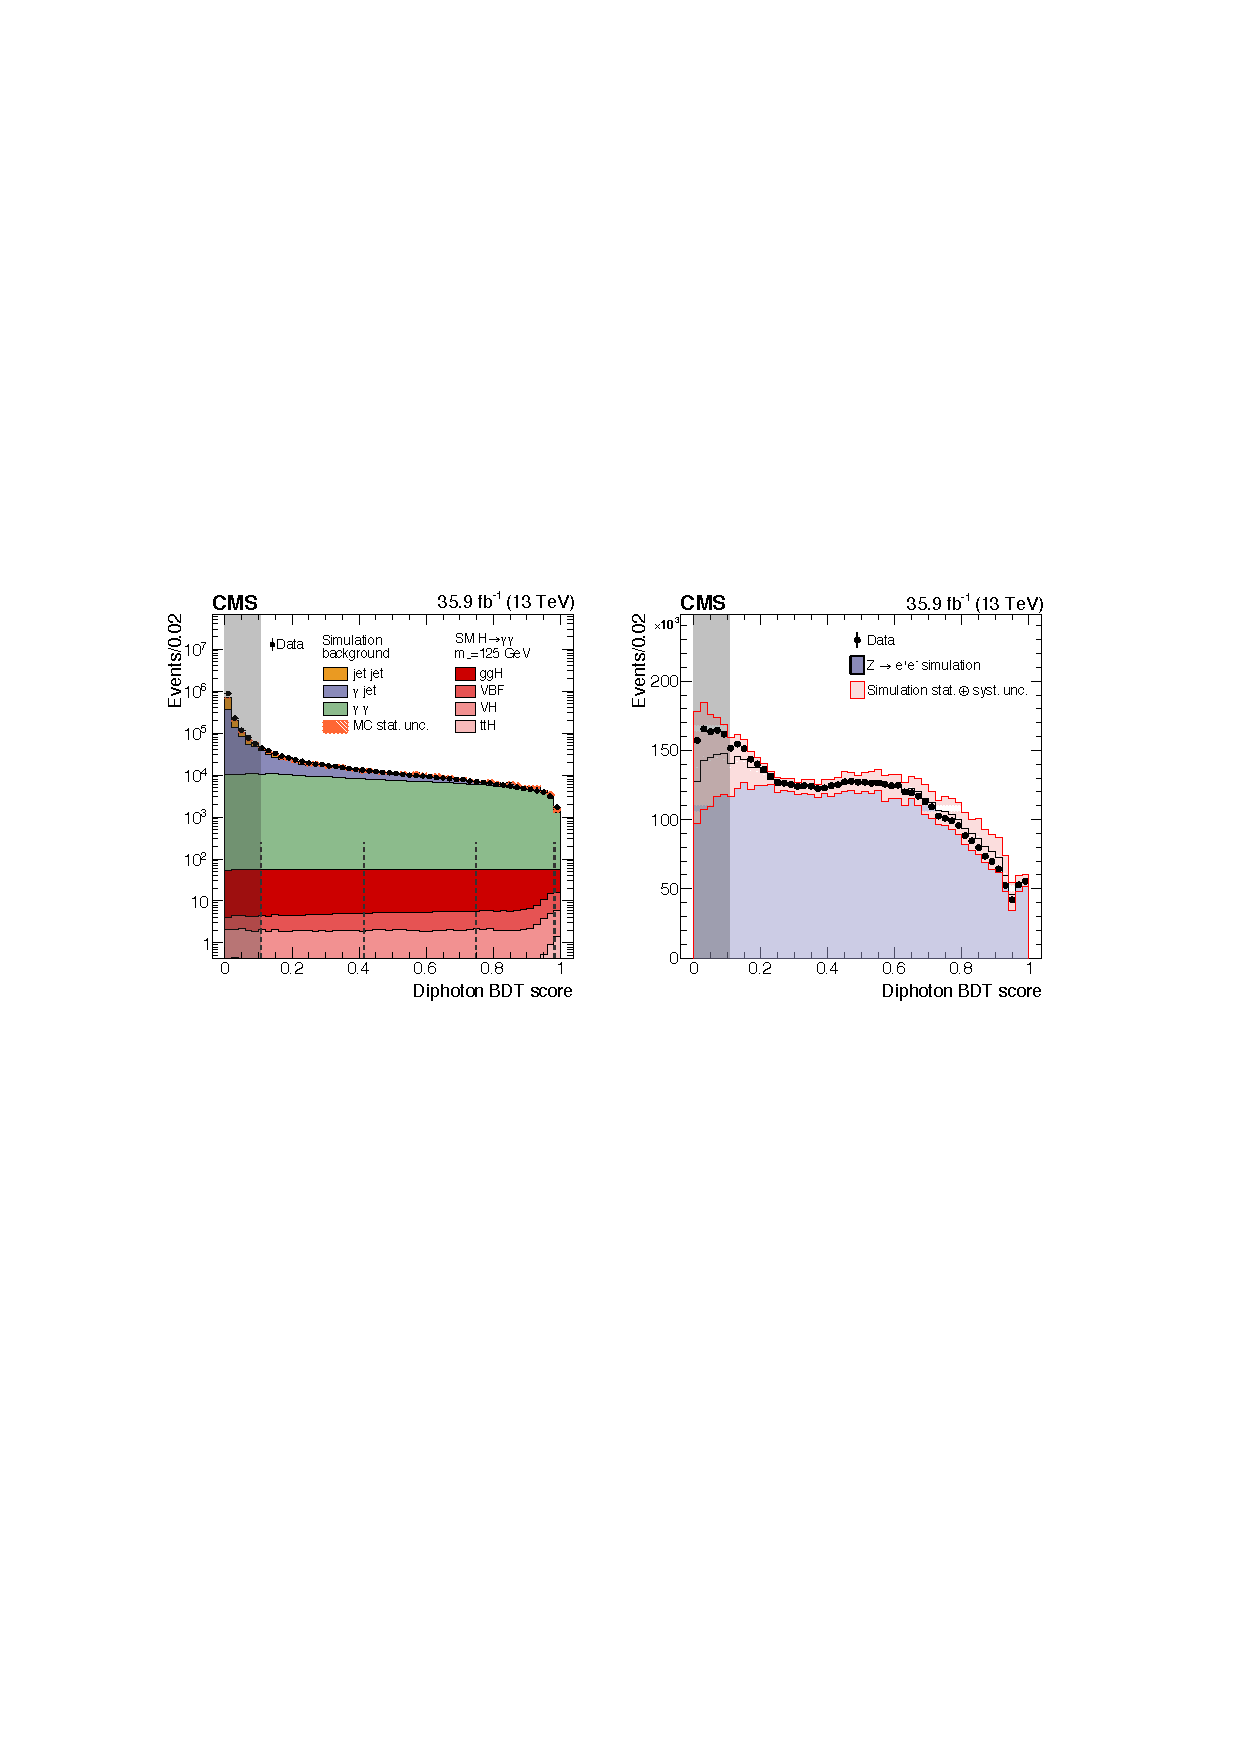
\includegraphics[width=0.99\textwidth]{figures/event_selection/diphoton_BDT.pdf}
    \caption{Stacked diphoton BDT score distributions for simulated signal and background, with data shown superimposed (left). Diphoton BDT score in the \Zee control region (right). 
             The same transformation has been applied to the score distribution in both plots such that the total signal distribution is flat.}
        \label{fig:event_categorisaton:diphoton_bdt}
\end{figure}


\subsection{Tagging Scheme}
Tagging is implemented as a fall-through sequence where diphoton events are offered to each tag in order of priority (Table \ref{tab:event_categorisaton:tag_sequence}). 
If a diphoton event is not accepted by a tag it then passes to the next tag for consideration until the final `untagged' tag category. 
If the event does not meet the criteria for this last tag it is discarded.
In the case of multiple tagged candidate diphotons in an event the one with the highest priority tag and category is selected, if they are in the same category the diphoton with the highest diphoton $p_{T}$ is chosen.
The criteria for each tag will be specified in following sections in this chapter.
\begin{table}[h!]
    \centering
    \resizebox{\linewidth}{!}{%
    \renewcommand{\arraystretch}{1.3}
    \begin{tabular}{ l | l l }
        \thickhline
        Tag & Target Process & Structure \\
        \hline
        \ttH Leptonic      & \ttH with semi-leptonic top decays & Single category \\
        \ttH Hadronic      & \ttH with fully-hadronic top decays & Single category \\
        ZH Leptonic        & VH with leptonically-decaying Z boson & Single category \\
        WH Leptonic        & VH with leptonically-decaying W boson & Single category \\
        VH Leptonic Loose  & VH with leptonically-decaying W or Z boson & Single category \\
        VBF                & VBF with dijet in the final state & Three categories \\
        VH MET            & VH with significant amount of \MET & Single category \\
        VH Hadronic        & VH with hadronically-decaying W or Z boson & Single category \\
        Untagged           & Inclusive & Four categories \\
        \thickhline
    \end{tabular}}
    \caption{The \Hgg tag sequence in order of tag priority from highest (top) to lowest (bottom).}
    \label{tab:event_categorisaton:tag_sequence}
\end{table}







\section{Top Fusion Tagging}
In the \ttH production mode, a top-antitop pair is produced in association with the Higgs boson. The top quark immediately decays to a b quark and a W boson which will subsequently decay leptonically or hadronically. In the former (semi-leptonic) case there will be a bottom quark jet plus an associated lepton with \MET from the W decay. In the latter (fully-hadronic) case there will be a bottom quark jet plus two quark jets from the W decay to quarks (Figure \ref{fig:event_categorisaton:top_decays}). 
\begin{figure}[h!]
    \begin{center}
        \begin{tikzpicture}[baseline=(current bounding box.center)]
        \begin{feynman}
            \vertex (a) {$t$};
            \vertex [right=of a] (b);
            \vertex [above right=of b] (f1);
            \vertex [below right=of b] (f2) {$b$};
            \vertex [above right=of f1] (f3) {$(u,c)$};
            \vertex [below right=of f1] (f4) {$(\bar{d},\bar{s},\bar{b})$};
            \diagram* {
                (a) -- [fermion] (b) -- [boson, edge label=\(W^{+}\)] (f1),
                (b) -- [fermion] (f2),
                (f1) -- [fermion] (f3),
                (f4) -- [fermion] (f1),
            };
        \end{feynman}
        \end{tikzpicture}
        %
        \qquad
        \begin{tikzpicture}[baseline=(current bounding box.center)]
        \begin{feynman}
            \vertex (a) {$t$};
            \vertex [right=of a] (b);
            \vertex [above right=of b] (f1);
            \vertex [below right=of b] (f2) {$b$};
            \vertex [above right=of f1] (f3) {${(\nu_{e},\nu_{\mu},\nu_{\tau})}$};
            \vertex [below right=of f1] (f4) {${(\bar{e},\bar{\mu},\bar{\tau})}$};
            \diagram* {
                (a) -- [fermion] (b) -- [boson, edge label=\(W^{+}\)] (f1),
                (b) -- [fermion] (f2),
                (f1) -- [fermion] (f3),
                (f4) -- [fermion] (f1),
            };
        \end{feynman}
        \end{tikzpicture}
    \end{center}
    \caption{Top quark decay modes: a fully-hadronic decay (left) and a semi-leptonic decay (right).}
    \label{fig:event_categorisaton:top_decays}
\end{figure}

The top tags target these two decay modes: the leptonic tag searches for \ttH events where at least one top quark decays semi-leptonically, and the hadronic tag searches for \ttH events where both top quarks decay fully-hadronically. 

\subsection{\ttH Leptonic}
This tag uses a set of selections on kinematic properties of leptons and jets in the event. 
Leptons are required to pass selection requirements depending on their flavour:
\begin{itemize}[noitemsep]
    \item diphoton BDT score $> 0.11$;
    \item at least one selected lepton with $p_{T} > 20$\,GeV;
    \item all selected leptons are required to have an angular separation from a signal photon of $R(\ell,\gamma) > 0.35$;
    \item $|m_{e\gamma} - m_{Z}| > 5$\,GeV (electrons only);
    \item a minimum of two jets in the event with $p_{T} > 25$\,GeV, $|\eta| < 2.4$, $R(j,\gamma) > 0.4$ and $R(j,\ell) > 0.4$;
    \item at least one jet is tagged as a b jet by the CSV tagger (medium requirement).
\end{itemize}


\subsection{\ttH Hadronic}
This tag uses a set of selections on kinematic properties of the jets in the event, as well as a dedicated BDT. The \ttH hadronic BDT is trained on the following input features:
\begin{itemize}[noitemsep]
    \item the number of jets with $p_{T} > 25$\,GeV;
    \item the $p_{T}$ of the leading jet;
    \item the two highest scores of the CSV b-tagger.
\end{itemize}
A selection on the BDT output score (Figure \ref{fig:event_categorisaton:tth_hadronic_bdt}) is optimised simultaneously on simulation with a selection on the diphoton BDT score to maximise expected precision on the signal strength of the \ttH production channel. 
\begin{figure}[h!]
    \centering
    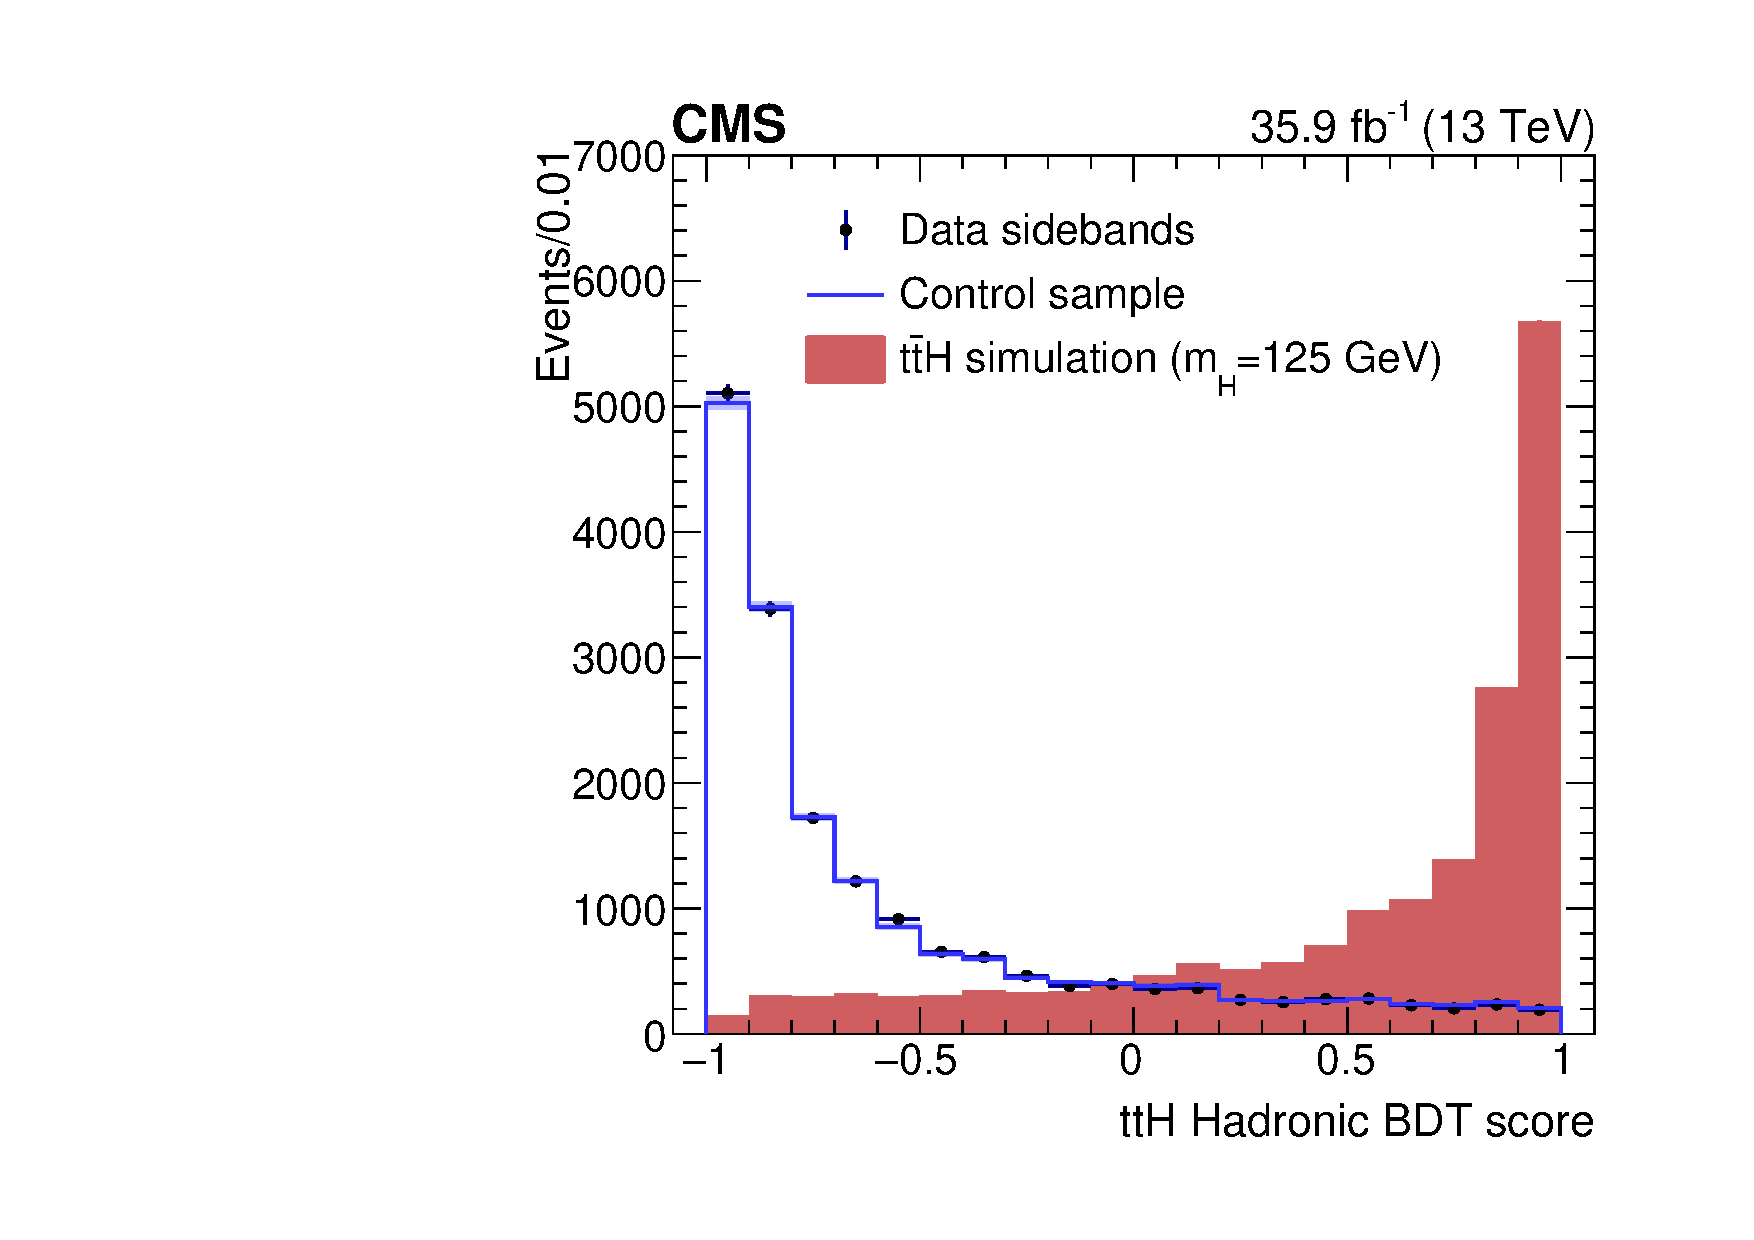
\includegraphics[width=0.5\textwidth]{figures/event_selection/CMS-HIG-16-040_Figure_006.pdf}
    \caption{Score distribution of the hadronic \ttH BDT. The blue lined histogram shows the distribution for the control region, the red filled histogram shows the score distribution for simulated signal, and the points show the score distribution of the data sideband regions ($m_{\gamma\gamma} < 115$\,GeV or $m_{\gamma\gamma} > 135$\,GeV).}
        \label{fig:event_categorisaton:tth_hadronic_bdt}
\end{figure}

A control region is constructed by selecting photon pairs where one passes the preselection and photon ID requirements, whilst the other has no preselection requirement and the photon ID is inverted.
These events are then weighted in $\eta$ and $p_T$ to reproduce the kinematic properties of the photons in the signal region.

The selection requirements of the \ttH Hadronic tag are as follows:
\begin{itemize}[noitemsep]
    \item $p_{T}/m_{\gamma\gamma} > 1/3$ and $1/4$ for leading and subleading photons respectively;
    \item diphoton BDT score $> 0.4$;
    \item no leptons that meet the criteria of the \ttH Leptonic tag;
    \item a minimum of three jets in the event with $p_{T} > 25$\,GeV and $|\eta| < 2.4$;
    \item at least one jet is tagged as a b jet by the CSV tagger (medium requirement);
    \item a \ttH Hadronic BDT score above 0.75.
\end{itemize}











\section[VH Tagging]{Associated Production Tagging}
In the associated production (VH) mode a W$^{\pm}$ or Z boson is produced in association with the Higgs boson. The VH tags target different vector bosons decaying in different ways which can manifest as leptons, jets or \MET in the event.
All of the leptonic VH tags are selection-based and have various isolation requirements to avoid contamination from Drell-Yan background processes.

\subsection{ZH Leptonic}
This tag targets Higgs production in association with a Z boson that subsequently decays leptonically with stringent requirements. The selection criteria are as follows:
\begin{itemize}[noitemsep]
    \item $p^{\gamma}_{T}/m_{\gamma\gamma} > 3/8$ for leading photon;
    \item diphoton BDT score $> 0.11$;
    \item two same-flavour leptons with $p_T > 20$\,GeV and satisfying the same requirements as in the \ttH Leptonic tag;
    \item $70 < m_{\ell\ell} < 110$\,GeV;
    \item $R(\gamma,e) > 1.0$, or $R(\gamma,\mu) > 0.5$;
    \item conversion electron veto: if an electron and a photon share a supercluster, the electron track must be well-separated from the supercluster centre ($R(SC,e) > 0.4$).
\end{itemize}


\subsection{WH Leptonic}
Targets Higgs production in association with a W$^{\pm}$ boson that subsequently decays leptonically with stringent requirements. The selection criteria are as follows:
\begin{itemize}[noitemsep]
    \item $p^{\gamma}_{T}/m_{\gamma\gamma} > 3/8$ for leading photon;
    \item diphoton BDT score $> 0.28$;
    \item at minimum one lepton with $p_T > 20$\,GeV and satisfying the same requirements as in the \ttH Leptonic tag;
    \item $R(\gamma,\ell) > 1.0$;
    \item \MET$> 45$\,GeV;
    \item a maximum of two jets each satisfying $p_T > 20$\,GeV, $|\eta|\, < 2.4$, $R(j,\ell) > 0.4$, $R(j,\gamma) > 0.4$;
    \item electron conversion veto as in the ZH Leptonic tag.
\end{itemize}



\subsection{VH Leptonic Loose}
This tag targets Higgs production in association with either W$^{\pm}$ or Z which then decay leptonically. 
This tag uses an orthogonal \MET selection of \MET$ < 45$\, GeV, with the rest of the selection being the same as WH Leptonic.

\subsection{VH MET}
Targets Higgs associated production with \MET from at least one missing lepton. The selection criteria are as follows:
\begin{itemize}[noitemsep]
    \item $p^{\gamma}_{T}/m_{\gamma\gamma} > 3/8$ for leading photon;
    \item diphoton BDT score $> 0.79$;
    \item \MET$> 85$\,GeV;
    \item $|\Delta\phi(\gamma\gamma,E_{T}^{miss})|\, > 2.4$.
\end{itemize}


\subsection{VH Hadronic}
This tag targets Higgs production in association with a W or Z boson that decays hadronically. The selection criteria are as follows:
\begin{itemize}[noitemsep]
    \item $p^{\gamma}_{T}/m_{\gamma\gamma} > 1/2$ for leading photon;
    \item diphoton BDT score $> 0.79$;
    \item a minimum of two jets with $p_T > 40$\,GeV and $|\eta|\, < 2.4$, $R(j,\gamma) > 0.4$;
    \item dijet invariant mass $60 < m_{jj} < 120$\,GeV;
    \item $|\mathrm{cos}{\theta^{*}}| \,< 0.5$, where $\theta^{*}$ is the difference in diphoton polar angles $\theta_{\gamma\gamma}$ in the diphoton-dijet centre-of-mass frame, and the lab frame.  
\end{itemize}




\section{Untagged}
If the candidate is not assigned to any of the other tags it is considered for inclusion in a final inclusive tag: Untagged. 
The Untagged tag consists of four categories defined as exclusive selections on the diphoton BDT score and consists mostly of gluon fusion events. 
If an event does not meet the lowest requirement it is discarded from the analysis.

These categories are optimised simultaneously in a similar way to the VBF tag, but with a few differences. 
The procedure begins with the boundaries spaced equally along the score distribution. Each category is evaluated in simulation by fitting an exponential for background plus two Gaussian distributions for the signal. 
Significance is extracted from each category based on a fit to an Azimov dataset derived from the earlier exponential and Gaussian function fits. 
The boundaries are optimised to maximise overall significance of the Untagged tag.

This procedure is repeated for increasing numbers of Untagged categories until there is no significant increase in performance. This is then the number of Untagged categories to be used in the tag.











\section{VBF Tagging}
The VBF production mode is characterised by its distinctive event topology and kinematics: two high-$p_{T}$ jets with large pseudorapidity separation and high invariant mass. Furthermore, the dijet substructure will also be distinctive with both jets originating from quarks, having colour connections to the proton remnants and possibly having other correlations in structure between the two jets. 

Other production modes can also produce a Higgs boson in association with jets to produce a VBF-like final state. 
In particular, ggH can be a significant source of background due to its larger cross section and capacity to produce jets at next-to-leading order or from initial-state radiation. 
These dijets will mostly be from gluons, therefore targeting the jet substructure will be important in discriminating these production modes. 


%Couple sentences on the tag and the two models
The VBF tag targets the VBF production mode by exploiting the distinctive properties of VBF dijets. 
At the core of the VBF tag is a machine learning model which takes these distinctive properties as input features. 
The selection and category assignment of the tag is then based on the output of this model.
This chapter explores two approaches.
\begin{itemize}[noitemsep]
    \item A tag based on two BDTs with engineered kinematic features using \texttt{Scikit-learn} \cite{SKLearn}. This is the approach used in the 2016 \Hgg analysis. 
    \item A tag based on a single dense convolutional neural network built in \texttt{TensorFlow} \cite{TensorFlow} that receives jet structure information in the form of images in addition to engineered kinematic features. 
\end{itemize}
Both tags use the same event preselection, and produce scores used to define event categories that enhance the expected significance of the VBF channel and will be evaluated in the same way. The only difference will be the machine learning model that the tags are based around, and the extra image-based information in the dense CNN tag.  

%Problem formulation of the ML part
The problem formulation is the following: to separate VBF from SM background and ggH events using simulated data. 
Constraints are that the model must generalise to real data and must not introduce a bias to the diphoton mass. 
There are a few challenges associated with this problem.
\begin{itemize}[noitemsep]
    \item There is a severe class imbalance where there are approximately seven times more examples of the background class than the signal.
    \item The events are weighted, some events can be equivalent to multiple others.
    \item Some events have negative weight and are needed for correct distribution shapes.
    \item The total weight difference between the classes is very large and make the class imbalance problem even worse.
    \item The QCD background sample has very large weights and very few events. This causes the background distribution shapes to become very jagged. 
\end{itemize}



%Figures of merit
%Models
The model is evaluated using the area under the ROC curve (AUROC), a performance measure of a binary classifier. 
This measure is chosen because it is robust to class imbalance and can easily be evaluated with weighted events.

%The Tag 
When developing the tag itself and its categories the approximate mean significance (AMS) \cite{HiggsML} is used as the figure of merit. This is defined as
\begin{equation}
    \mathrm{AMS} = \sqrt{2\left( (s+b+b_{\mathrm{reg}})\log\left(1 + \frac{s}{b+b_{\mathrm{reg}}}\right) - s \right)},
\end{equation}
where $s$ is the total number of signal events, $b$ is the total number of background events, and $b_{\mathrm{reg}}$ is a regularisation term that reduces sensitivity to local optima. 
The value of $b_{\mathrm{reg}}$ is chosen to be 5. 
$\mathrm{AMS}$ is estimated by simultaneously fitting an exponential plus a double Gaussian function to the diphoton mass distribution. 
The background and signal event weights from an interval of two effective standard deviations around the peak are summed to produce $s$ and $b$, and to estimate $\mathrm{AMS}$. 







\subsection{Selections}
When a candidate diphoton is considered for VBF selection additional requirements are applied based on the jet content of the event. First requirements are applied on a per-jet basis, if there are more than two jets which meet these requirements the top two in $p_{T}$ are selected to form a dijet. Finally, a preselection based on dijet kinematics is applied to the candidate dijet. If it does not pass, the event falls through to the lower-priority categories (VH MET, VH Hadronic, and Untagged). 

\subsubsection{Jet Selection}
Jets are required to meet the criteria detailed in the previous chapter plus some additional requirements specific to the VBF tag.
Pileup jet ID (PUJID) uses a BDT classifier \cite{CMS-PAS-JME-13-005} that takes a collection of jet shape variables and produces a score for each jet. A collection of selections on this score are then applied for bins in $p_{T}$ and $\eta$ (Table \ref{tab:event_selection:tight_pujid}). 
\begin{table}[h!]
    \centering
    \renewcommand{\arraystretch}{1.3}
    \begin{tabular}{ l | c c c c }
        \thickhline
         & $|\eta| < 2.5$ & $2.5 \leq |\eta| < 2.75$ & $2.75 \leq |\eta| < 3.0$ & $3.0 \leq |\eta| < 5.0$ \\
        \hline
        $20 < p_{T} \leq 30$\,GeV  & $0.69$ & $-0.35$ & $-0.26$ & $-0.21$ \\
        $30 < p_{T} \leq 50$\,GeV  & $0.86$ & $-0.10$  & $-0.05$ & $-0.01$ \\
        $50 < p_{T} \leq 100$\,GeV & $0.95$ & $0.28$  & $0.31$  & $0.28$  \\
        \thickhline
\end{tabular}
    \caption{Pileup jet ID cuts of the tight working point.}
    \label{tab:event_selection:tight_pujid}
\end{table}
In this analysis the tight working point is used as this gives the highest expected significance for the VBF tag, and also leads to marked improvement in data/simulation agreement in $\eta$ in the \Zee plus jets control region.  
Furthermore there is a photon-jet isolation criterion that requires the jet to have $\Delta{R}(\gamma,j) > 0.4$ with both of the photons of the candidate diphoton and a jet pseudorapidity requirement of  $|\eta_{j}| < 4.7$.







\subsubsection{Dijet Preselection}
Dijets are formed by selecting the two highest-$p_T$ jets in the event that pass the jet selection requirements. The highest-$p_T$ jet in the pair is referred to as the leading jet, and the other jet as the subleading jet. If there are fewer than two jets the event is rejected by the VBF tag and falls through to untagged. 
Candidate dijets are required to meet the following selection criteria before being presented to the machine learning model:
\begin{itemize}[noitemsep]
    \item $p^{\gamma}_{T}/m_{\gamma\gamma} > 1/3$ and $1/4$ for leading and subleading photon respectively;
    \item photon ID BDT score $> -0.2$ for both photons;
    \item dijet invariant mass $m_{jj} > 250$\,GeV;
    \item jet $p_{T} > 40$\,GeV and $> 30$\,GeV for the leading and subleading jets respectively.
%    \item absolute pseudorapidity $|\eta| < 4.7$ for both jets.
\end{itemize}

The criterion on the photon ID score is motivated by under-performance of the diphoton BDT in the VBF phase space. 
The diphoton BDT was trained over all signal, the bulk of which will consist of ggH where the diphoton is produced with no extra objects such as jets. 
In this phase space the transverse momentum of the diphoton system is highly discriminating. 
This leads the diphoton BDT to assign a high score just on high values of diphoton $p_T$, and with lax requirements on photon ID. 
This in turn leads to under-performance in the VBF phase space where the $p_T$ spectrum is harder and low photon ID background events are given a high score. 








\section{VBF Tag with BDTs}
Once a candidate event passes the preselection it is presented to a machine learning model consisting of two BDTs in sequence: the dijet BDT and the combined BDT. 
The output classification score of this model will be used to define the categories of the tag selection. 

\subsection{Dijet BDT}
The purpose of the dijet BDT is to evaluate how VBF-like events are based on kinematic information from the dijet and the diphoton, and in particular to handle the rejection of ggH.
The BDT receives the following features which are chosen to minimise correlation with the diphoton mass:
\begin{itemize}[noitemsep]
    \item $p^{\gamma}_{T}/m_{\gamma\gamma}$ for the leading and subleading photons;
    \item $p_{T}^{j1}$ and $p_{T}^{j2}$, the transverse momenta of the leading and subleading jets respectively;
    \item $m_{jj}$ the invariant mass of the dijet;
    \item $\Delta\eta$ the pseudorapidity gap between the two jets;
    \item $\mathrm{min}\Delta{R}(\gamma,j)$ the smallest angular separation between either of the diphoton photons and either of the jets;
    \item $|\Delta\phi_{\gamma\gamma{jj}}|$ the absolute azimuthal angular difference between the diphoton and dijet;
    \item $|\Delta\phi_{jj}|$ the absolute azimuthal angular difference between the jets of the dijet;
    \item $C_{\gamma\gamma}$ the diphoton centrality expressed as:
        \begin{equation}
            C_{\gamma\gamma} = \mathrm{exp}\left(-\frac{4}{(\eta_{j1} - \eta_{j2})^{2}}\left( \eta_{\gamma\gamma} - \frac{\eta_{j1} + \eta_{j2}}{2} \right)^{2}\right)
        \end{equation}
        where $\eta_{j1}$ and $\eta_{j2}$ are the pseudorapidities of the leading and subleading jets.
\end{itemize}
Their distributions with the VBF preselection applied are shown in Figure \ref{fig:event_categorisaton:dijet_bdt_features}.
%\newpage

\begin{figure}[h!]
    \centering
    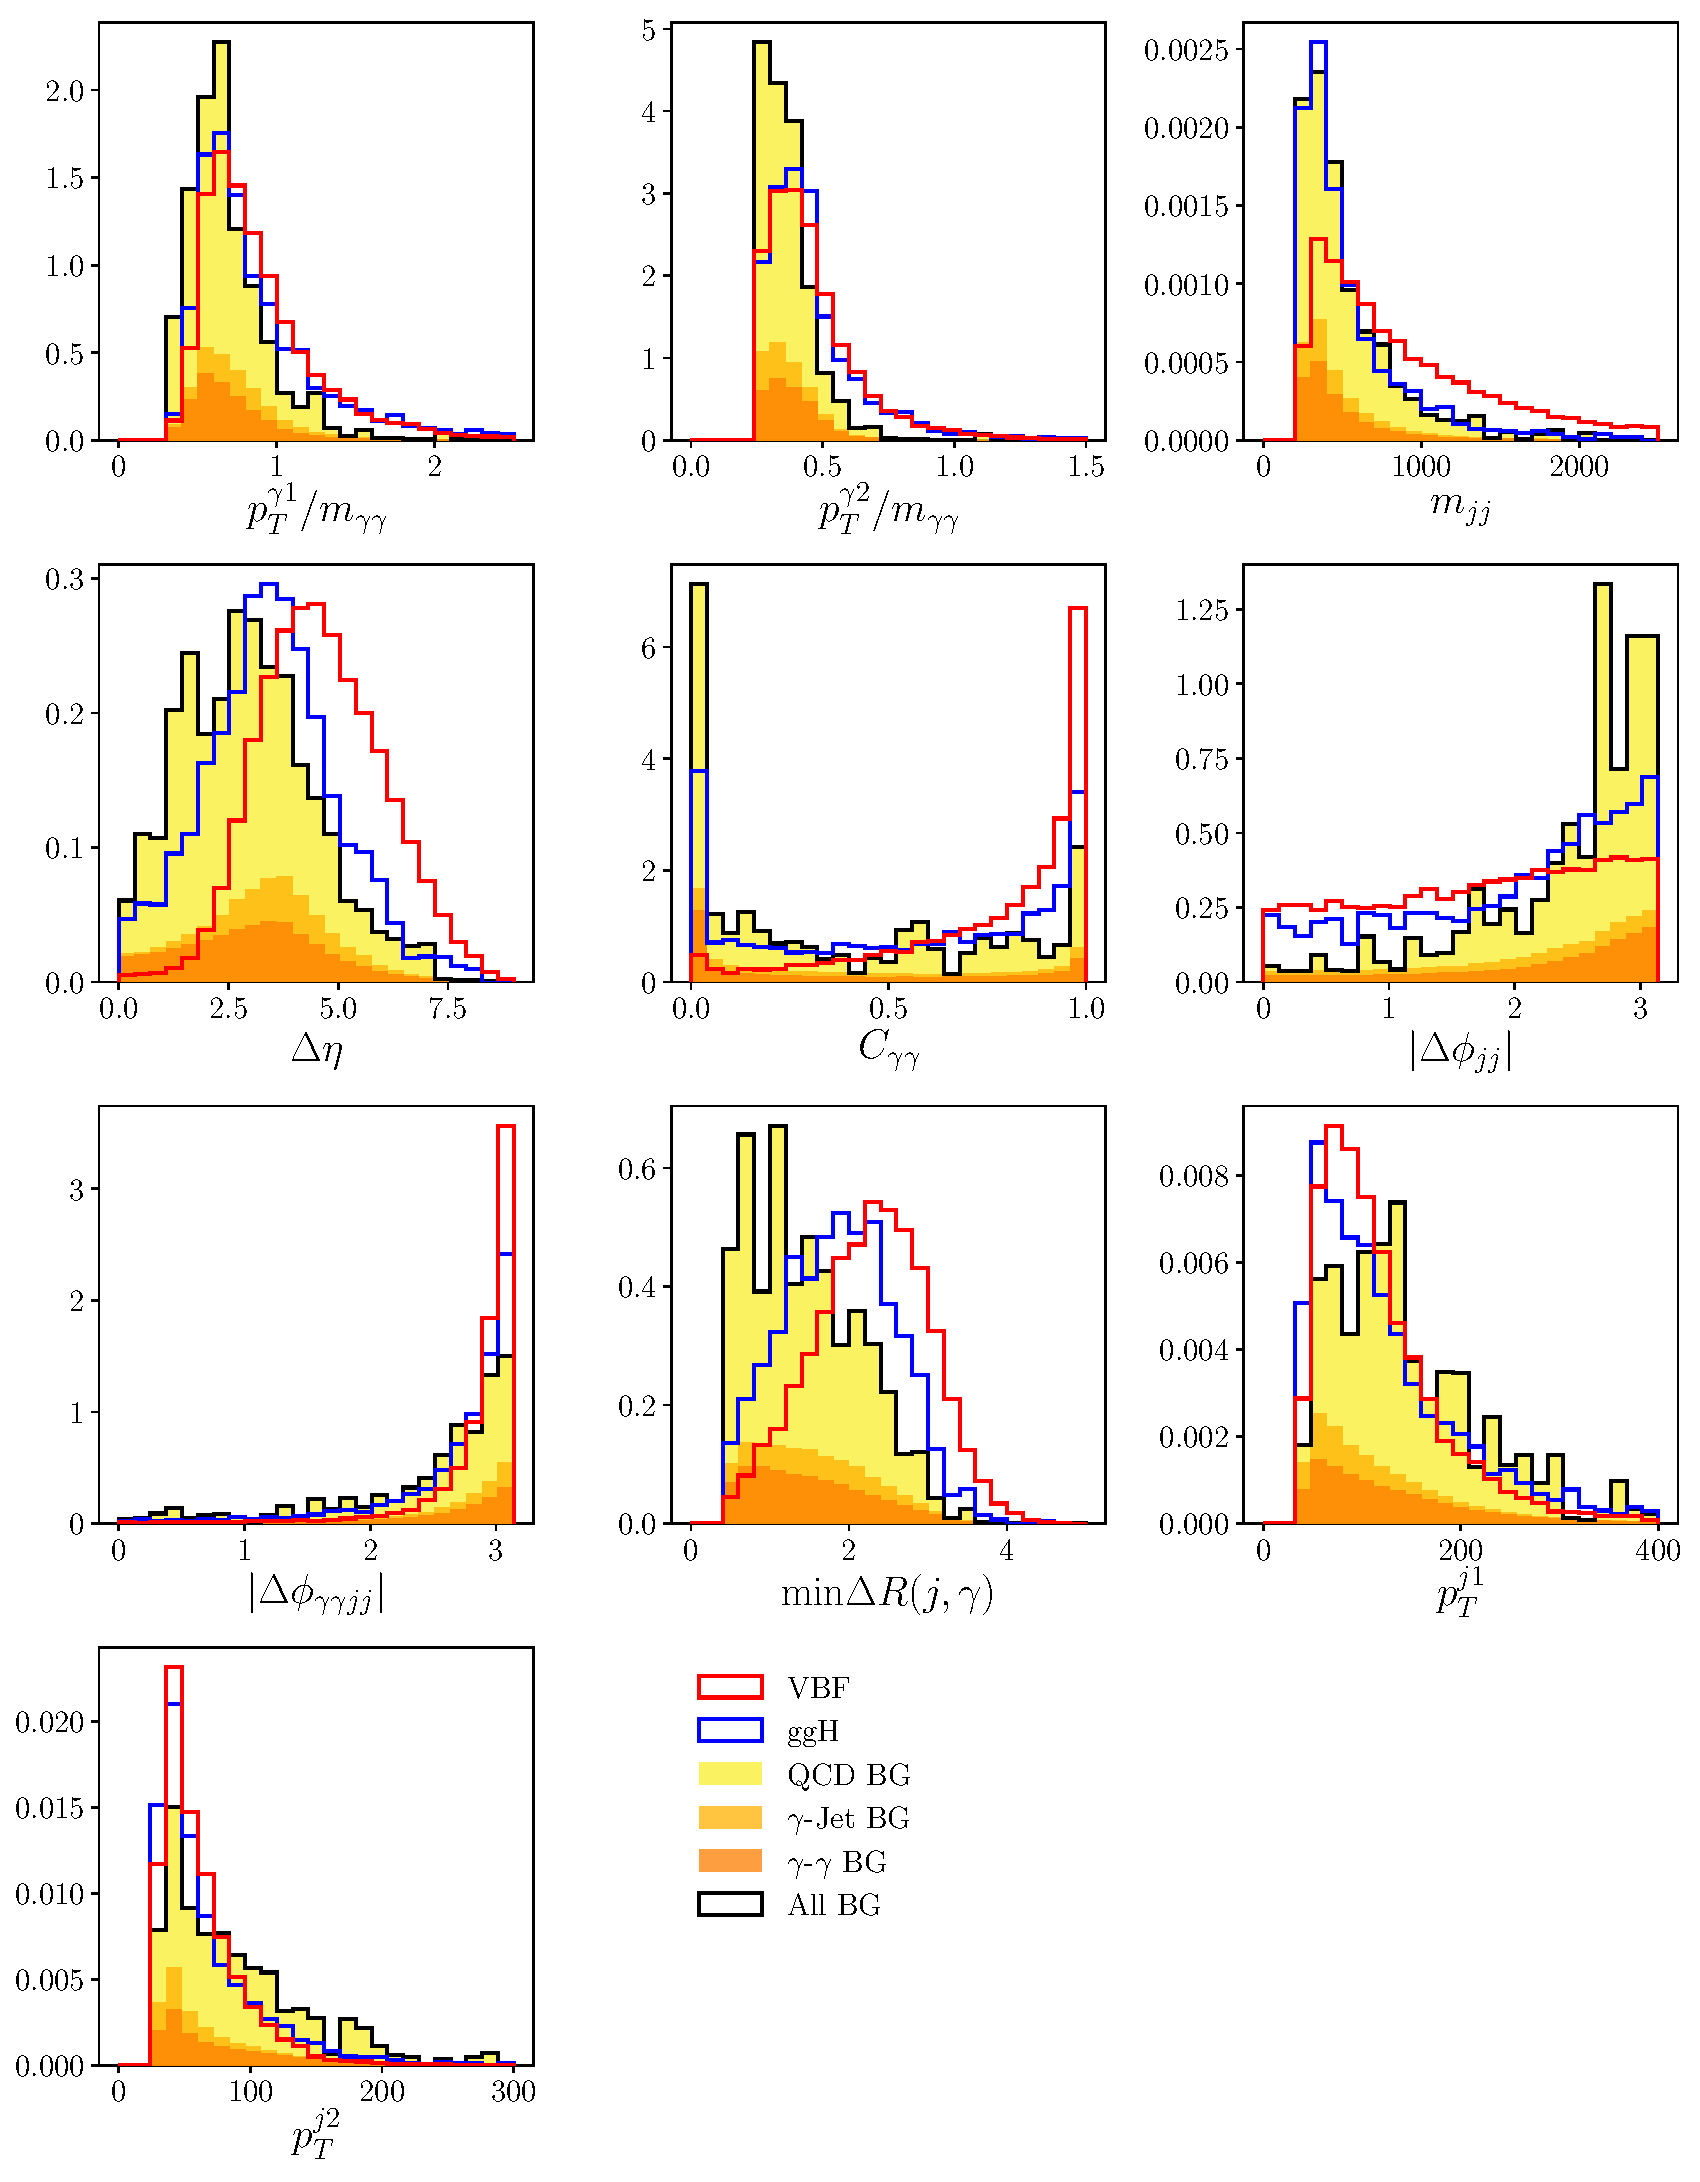
\includegraphics[width=0.99\textwidth]{figures/event_selection/dijet_BDT_features_splitBG_PS.pdf}
    \caption{Dijet BDT feature distributions with the full VBF preselection. Distributions are all normalised to unity with the solid red line corresponding to VBF, blue line to ggH, and black line to SM background. The SM background distribution is shown as a stacked histogram.}
    \label{fig:event_categorisaton:dijet_bdt_features}
\end{figure}


This dijet BDT is trained on all simulated SM background samples (with ggH included) versus VBF. To increase the number of training examples the training uses a loosened dijet preselection requirement where the $p_{T}^{\gamma}/m_{\gamma\gamma}$ are reduced to $1/4$ and $1/5$, the jet $p_T$ cuts are reduced by 10\,GeV, the dijet invariant mass cut is reduced to 100\,GeV and the photon ID cuts are not applied.
The normalised score distributions for the classes and the ROC curves for each individual sample are shown in Figure \ref{fig:event_categorisaton:dijet_bdt_performance}.
These scores are then used as an input feature in the next BDT in the VBF tag: the combined BDT. 
\begin{figure}[h!]
    \centering
        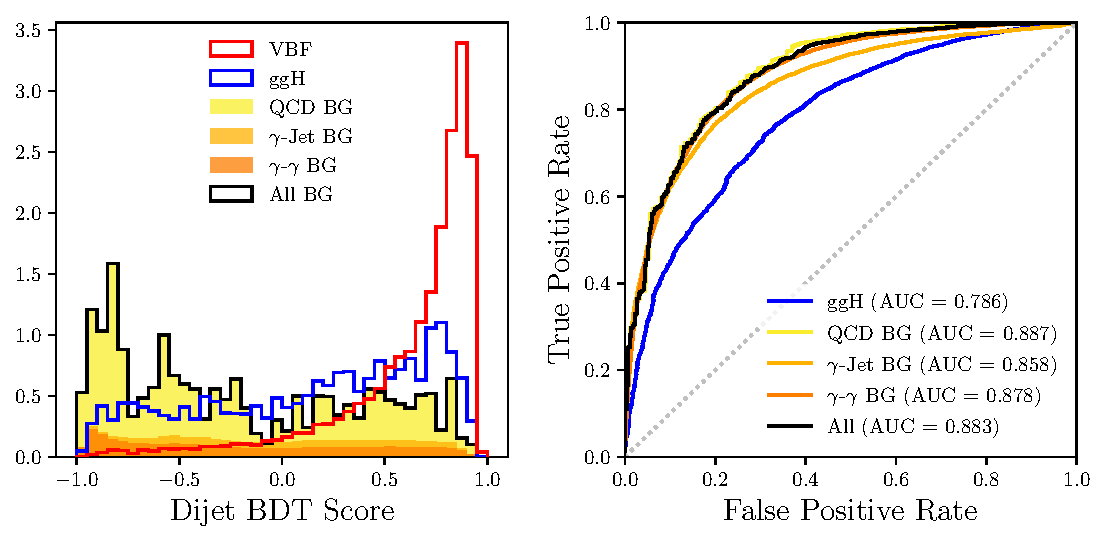
\includegraphics[width=0.8\textwidth]{figures/event_selection/dijet_BDT_PS.pdf}
    \caption{Dijet BDT performance. On the left are the output score distributions for VBF (red), ggH (blue) and SM background (black). The SM background distribution is shown as a stacked histogram. On the right are the ROC curves for the dijet BDT split into the different samples. The performance against ggH is noticeably lower than the other backgrounds.}
    \label{fig:event_categorisaton:dijet_bdt_performance}
\end{figure}









\subsection{Combined BDT}
The purpose of the combined BDT is to combine information from the diphoton BDT and dijet BDT to produce the final discriminant score for defining VBF tag categories. 
Specifically, it takes the following input features:
\begin{itemize}[noitemsep]
    \item diphoton BDT score;
    \item dijet BDT score;
    \item $p_{T}^{\gamma\gamma}/m_{\gamma\gamma}$, the mass-scaled transverse momentum of the diphoton.
\end{itemize}
The distributions of these features with the full VBF preselection applied are shown in Figure \ref{fig:event_categorisaton:combined_bdt_features}.
\begin{figure}[h!]
    \centering
    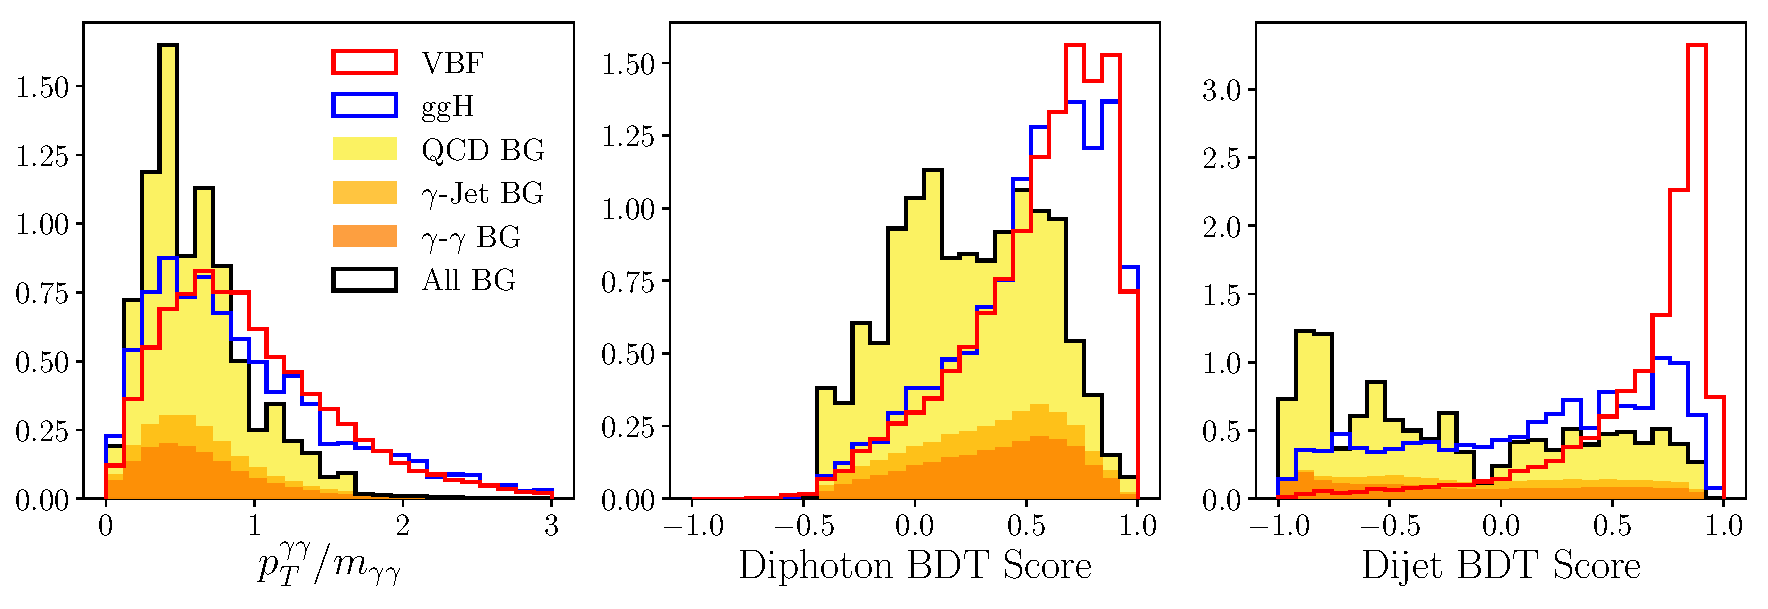
\includegraphics[width=0.99\textwidth]{figures/event_selection/combined_BDT_features_splitBG_PS.pdf}
    \caption{Combined BDT feature distributions with the full VBF preselection. Distributions are all normalised to unity with solid red corresponding to VBF, blue line to ggH. The SM background is shown as a stacked histogram.}
    \label{fig:event_categorisaton:combined_bdt_features}
\end{figure}

The combined BDT is then trained with the SM background samples vs VBF. Gluon fusion is not included in this training as it is found to reduce the ability of this BDT to reject SM background. This is considered to be a higher priority than ggH rejection because rejection of SM background has the largest impact on statistical significance.
The normalised combined score distributions for the classes and the ROC curves for each individual sample are shown in Figure \ref{fig:event_categorisaton:combined_bdt_performance}.
\begin{figure}[h!]
    \centering
        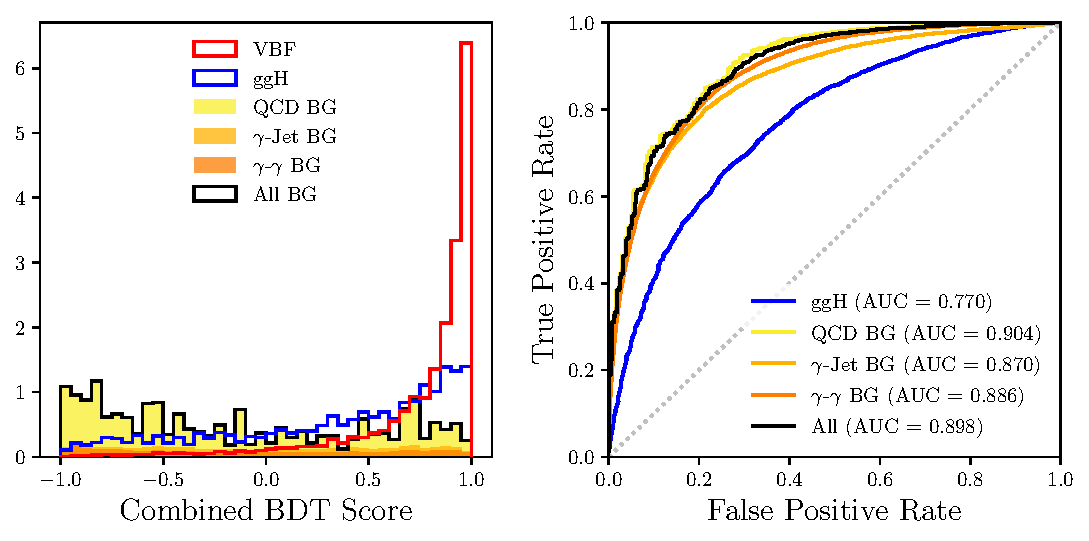
\includegraphics[width=0.8\textwidth]{figures/event_selection/combined_BDT_PS.pdf}
    \caption{Combined BDT score distribution with the full VBF preselection are shown on the left. Distributions are all normalised to unity with solid red corresponding to VBF, blue line to ggH, and black line to SM backgrounds. The SM background distribution is shown as a stacked histogram. ROC curves broken down by background sample are shown in the same colours on the right.}
    \label{fig:event_categorisaton:combined_bdt_performance}
\end{figure}



\subsection{Model Interpretation}
The model can be interpreted by observing how features are used together in high and low-scoring events. This is achieved by examining their joint distribution for highest and lowest percentile scoring events. 
The result is shown in Figure \ref{fig:event_categorisaton:bdt_based_vbf_tag_interpretation} where the solid colour shows the values averaged over each percentile, and the lines show the top five highest (or lowest) scoring events.
\begin{figure}[h!]
    \centering
    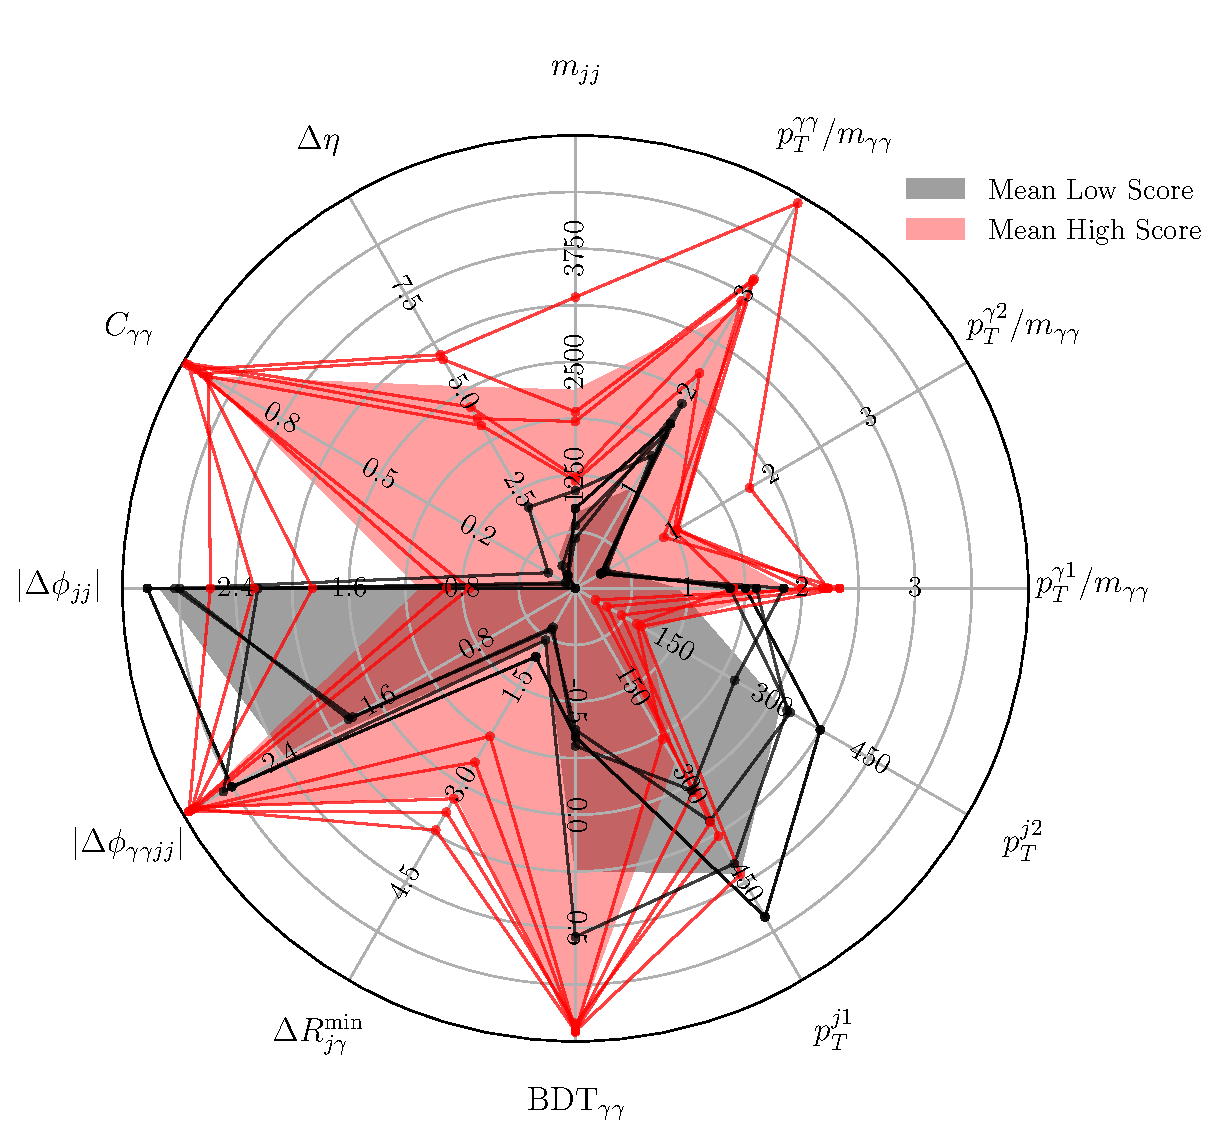
\includegraphics[width=0.65\textwidth]{figures/event_selection/eng_feature_radar_BDT.pdf}
    \caption{Coloured regions correspond to mean values for top percentile (red) and bottom percentile (black) combined score events. 
             The top and bottom five scoring events are also shown by lines and dots.}
    \label{fig:event_categorisaton:bdt_based_vbf_tag_interpretation}
\end{figure}

%Some generic comments
The discrimination power of the model is driven by the dijet angular variables, with the exception of $|\Delta\phi_{\gamma\gamma{jj}}|$ and the dijet mass.
High jet \pt is actually more of an indicator of background.
Diphoton BDT score shows substantial overlap, likely from ggH but there could still be residual high-\pt SM background events and underperformance in the VBF phase space.


\subsection{Categorisation and Tag Performance}
Once a candidate event has been preselected and evaluated by the model it is considered for inclusion in the VBF categories. 
These are defined as exclusive selections on the combined BDT output score and are chosen to maximise the $\mathrm{AMS}$ over all categories. 
If the combined score is not high enough for inclusion in the lowest category it is rejected and is passed for consideration by lower-priority tags. 

The $\mathrm{AMS}$ is estimated for each category by constructing a diphoton mass histogram of all events in the category score range, an exponential function is then fitted to the mass sidebands, and a double Gaussian in the signal region to the background-subtracted mass histogram. The parameters of these fits are then used as initial values for a simultaneous signal-background fit. 
The values of $s$ and $b$ are evaluated in a region around the peak with width equal to two effective sigma either side estimated from the the simultaneous fit. Overall significance is then calculated as the sum in quadrature of the significance of each category. 

The boundaries are optimised simultaneously for overall significance with a random search algorithm. The number of categories is chosen considering an increasingly larger number and performing a category optimisation for each one. The procedure stops when the improvement is less than one percent. This was found to happen with three categories. 

Approximate studies (in lieu of the full final fits machinery) of the three VBF categories using the procedure described above are carried out to study tag performance. Their boundaries and their estimated performance is shown in Figure \ref{fig:event_categorisaton:bdt_mass_fits} and Table \ref{tab:event_selection:legacy_cats}.
\begin{figure}[h!]
    \centering
    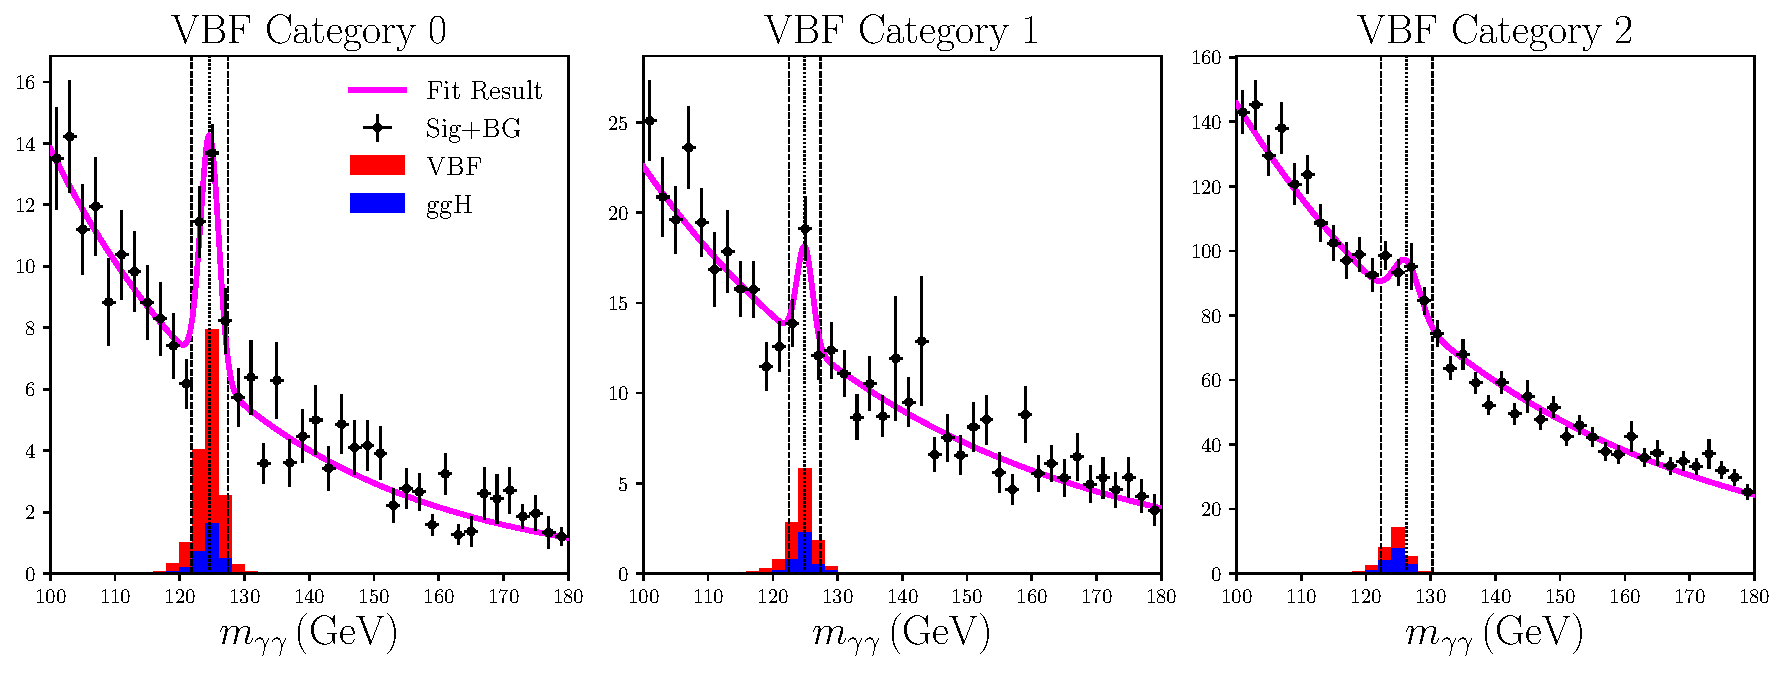
\includegraphics[width=1.0\textwidth]{figures/event_selection/BDT_mass_fits.pdf}
    \caption{Mass fits for estimating AMS.}
    \label{fig:event_categorisaton:bdt_mass_fits}
\end{figure}
\begin{table}[h!]
    \centering
    \renewcommand{\arraystretch}{1.3}
    \begin{tabular}{ l | c c c c c }
        \thickhline
        Category & Score Range & $\sigma_{\mathrm{eff}}$ & AMS & $B_{\mathrm{ggH}}/(S+B_{\mathrm{ggH}})$ & $S/(S+B)$ \\
        \hline
        VBF 0 & $[1.00, 0.957)$     & 1.4 &  2.16 & 0.20 & 0.37 \\
        VBF 1 & $[0.957, 0.902)$ & 1.2 &  1.00  & 0.34 & 0.17 \\
        VBF 2 & $[0.902, 0.553)$ & 2.0 &  0.69 & 0.53 & 0.04 \\
        \thickhline
    \end{tabular}
    \caption{Estimated category attributes for the BDT-based VBF tag.}
    \label{tab:event_selection:legacy_cats}
\end{table}






\subsection{Validation}
\subsubsection{\Zee Control Region}
Validation of the VBF tag uses the same \Zee control region as the other tags, but with the extra requirements of the VBF preselection. 
This control region is used for simulation/data comparison of both the features input to the BDTs and the BDT scores themselves (Figure \ref{fig:event_categorisation:zee_bdt_score_validation}). 
\begin{figure}[h!]
    \begin{center}
        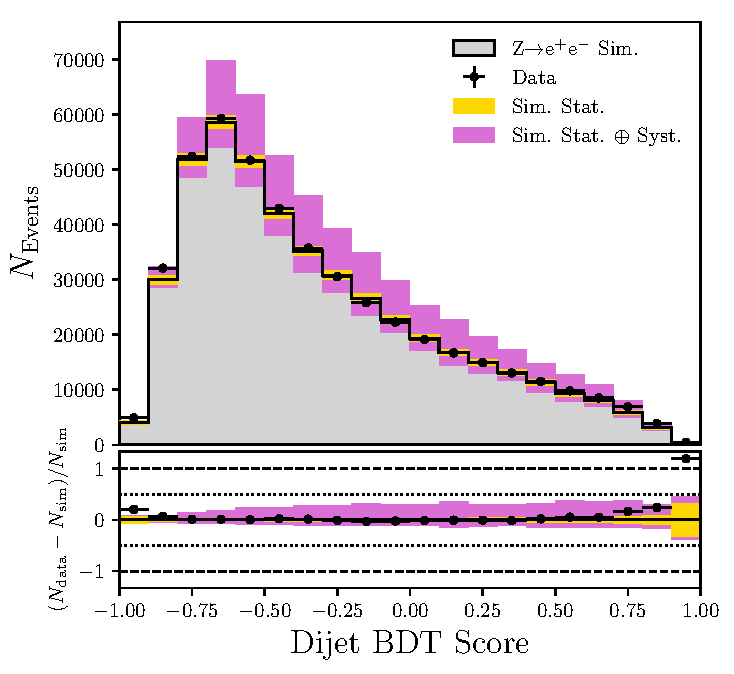
\includegraphics[width=0.49\textwidth]{figures/event_selection/dijet_BDT_zee_LPS.pdf}
        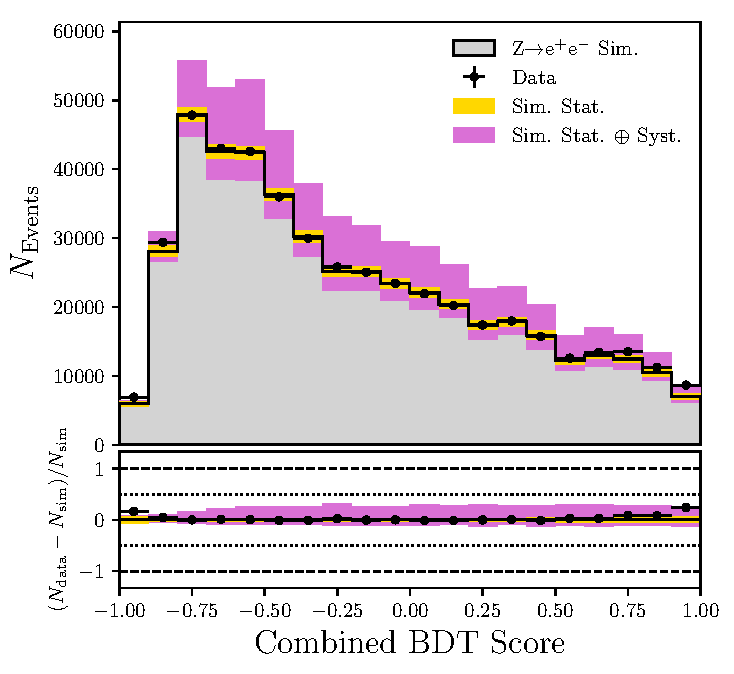
\includegraphics[width=0.49\textwidth]{figures/event_selection/combined_BDT_zee_LPS.pdf}
    \end{center}
    \caption{Data/Simulation comparison for dijet and combined BDT output scores.}
    \label{fig:event_categorisation:zee_bdt_score_validation}
\end{figure}
There is good data-simulation agreement in the output scores of the BDTs and in the kinematic features (Appendix \ref{appendix:vbf_zee}).


These plots only show the marginal distributions of these variables, they do not show their joint behaviour. 
To examine data-simulation agreement of the joint distribution a BDT is trained to discriminate between simulation and data events. 
If the discrimination power of the resulting model is high then the agreement is bad, if it is equivalent to guessing this suggests that the joint distributions match closely. 
Selections on the BDT score can then be used to try to isolate regions of the joint distribution where there is disagreement. 

The results shown in Figure \ref{fig:event_categorisation:zee_bdt_validation} show that the score distributions are similar, discrimination is very low, and therefore the joint feature distribution has little disagreement.
\begin{figure}[h!]
    \begin{center}
    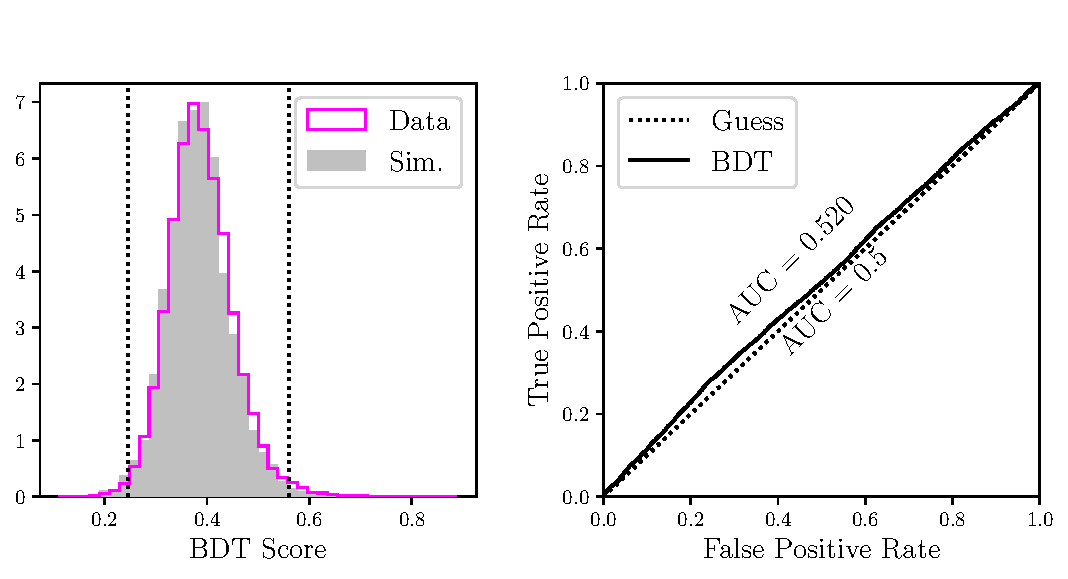
\includegraphics[width=0.9\textwidth]{figures/event_selection/eng_feature_ROC_Zee_BDT.pdf}
%    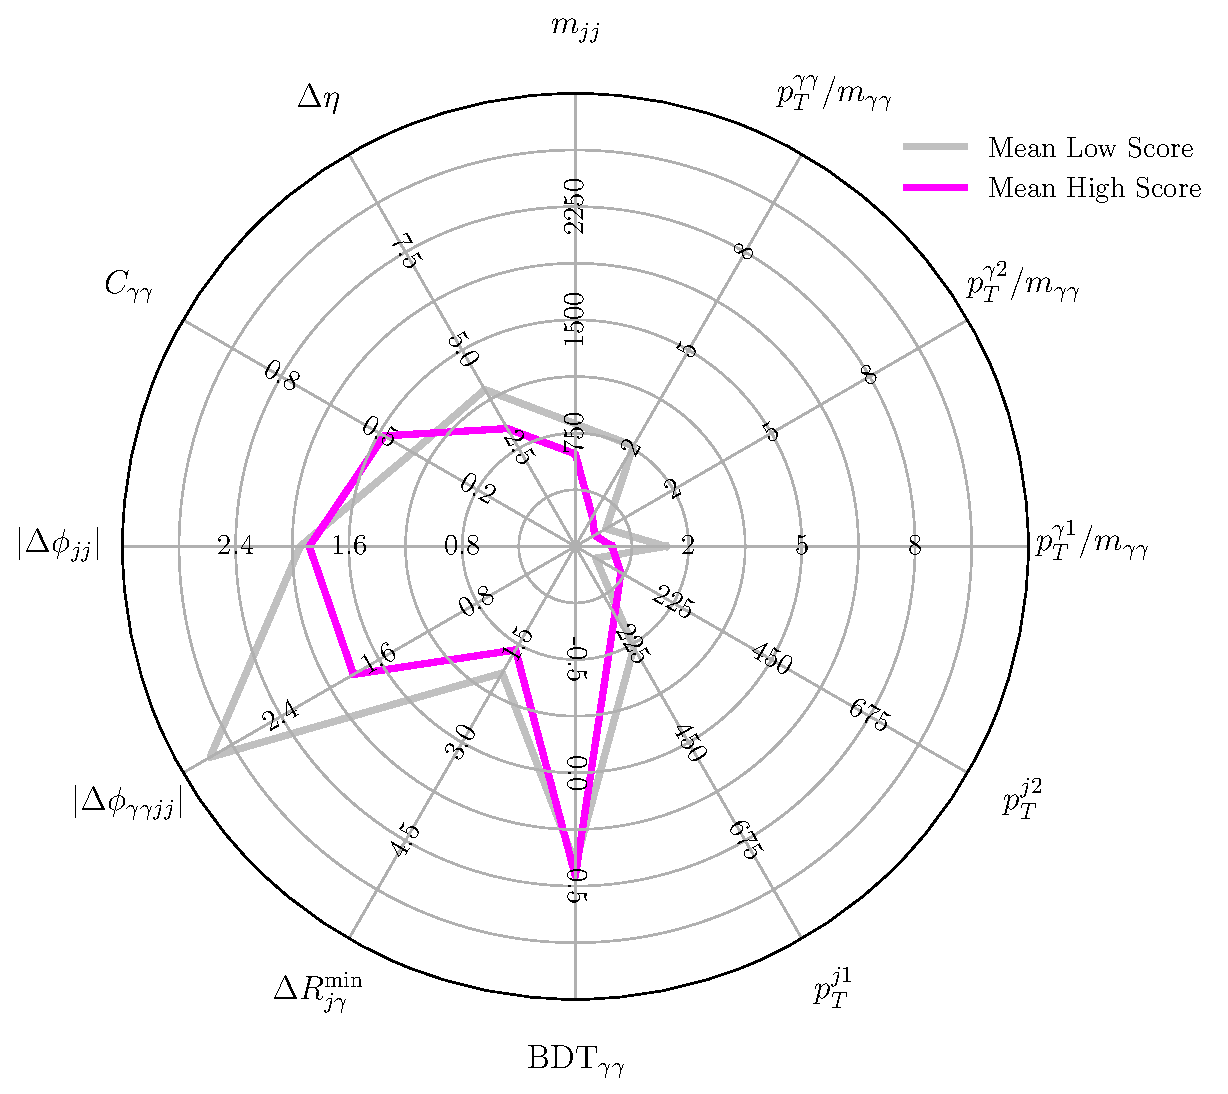
\includegraphics[width=0.6\textwidth]{figures/event_selection/eng_feature_radar_Zee_BDT.pdf}
    \end{center}
    \caption{Joint distribution study with BDT on the \Zee control region data-simulation test set.}
    \label{fig:event_categorisation:zee_bdt_validation}
\end{figure}


\subsubsection{QCD Modelling Variations}
The accuracy of QCD process modelling in hadronic collisions is a significant source of theoretical uncertainty. 
This will have an impact on categorisation with hadronic objects such as jets, and is especially pertinent for any features that are based on jet substructure. 

To test for how such mismodelling affects the VBF tag and VBF/ggH discrimination, samples are evaluated with up and down variations on aspects of jet production:
\begin{itemize}[noitemsep]
    \item \textbf{Underlying event}: interactions between parton pairs in the proton collision that are not part of the hard scatter;
    \item \textbf{Parton shower}: simulates a succession of parton emissions from the incoming and outgoing partons of the interaction.
\end{itemize}
Both of these will affect the cross section for jet production, the configuration of the jet substructure and particularly the degree of colour connection to the proton remnant.

To evaluate how the performance of the model changes depending on the QCD modelling, a ROC curve is constructed for each variant, and an envelope is drawn around the curves to estimate performance bounds. This is shown in figure \ref{fig:event_categorisation:ps_variant_validation}
\begin{figure}[h!]
    \begin{center}
        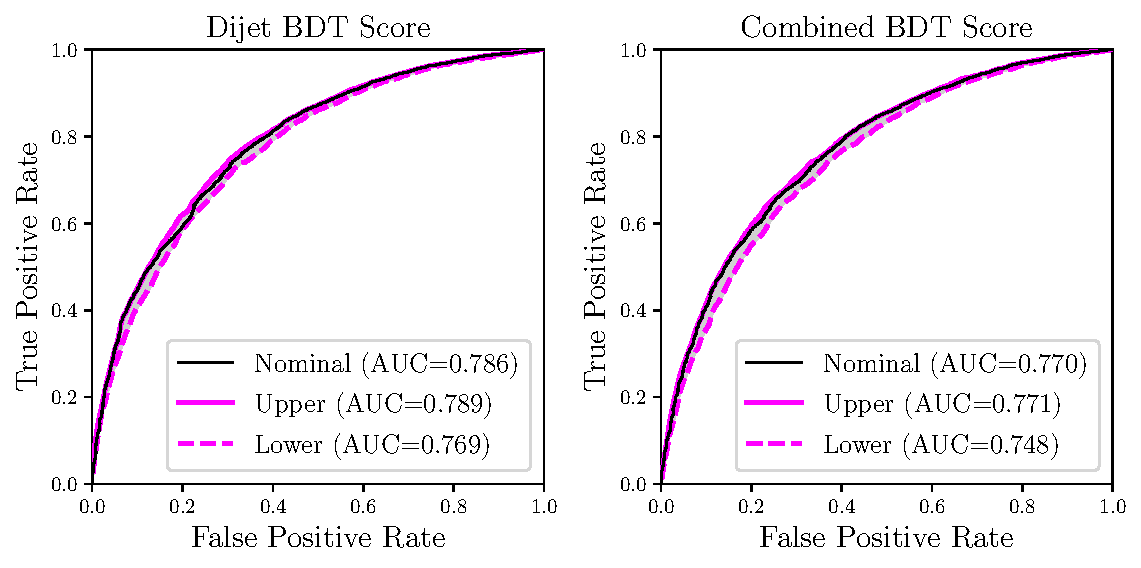
\includegraphics[width=0.9\textwidth]{figures/event_selection/psvar_ROCs_PS.pdf}
    \end{center}
    \caption{ROC curves for parton shower and underlying event variations. The nominal performance is shown in black, 
             and the magenta lines show the upper and lower bounds of the envelope covering all the curves.}
    \label{fig:event_categorisation:ps_variant_validation}
\end{figure}

The change in performance is modest. This is expected as the VBF model only uses kinematic variables, and the main impact of these variations may be through pileup mitigation and selecting the incorrect jet rather than substructure mismodelling. 


\subsection{Single BDT Model}
The two-step structure of the VBF tag was first developed for the Higgs boson Run 1 analysis  on less performant software and different selections. 
In particular, the photon ID cut of the preselection removes much of the background that the combined BDT targets. 
When trained over events with this cut applied, the combined BDT adds little to the performance of the VBF Tag. 
Using a single BDT equivalent to simply adding the diphoton BDT score to the dijet BDT performs at the same level as the two step tag (Figure \ref{fig:event_categorisation:single_BDT}).

Furthermore, the original train-test split of the two-step BDT was unavailable. Evaluating over the entire sample will include training events and exaggerate the performance of the BDT-based tag. 
A single-step BDT was trained and found to be equal in performance. A small increase in the two-step tag is possibly from the inclusion of training events. 
It is a fairer test to compare this model to the dense CNN because the exact same training and test sets can be used. 
\begin{figure}[h!]
    \centering
    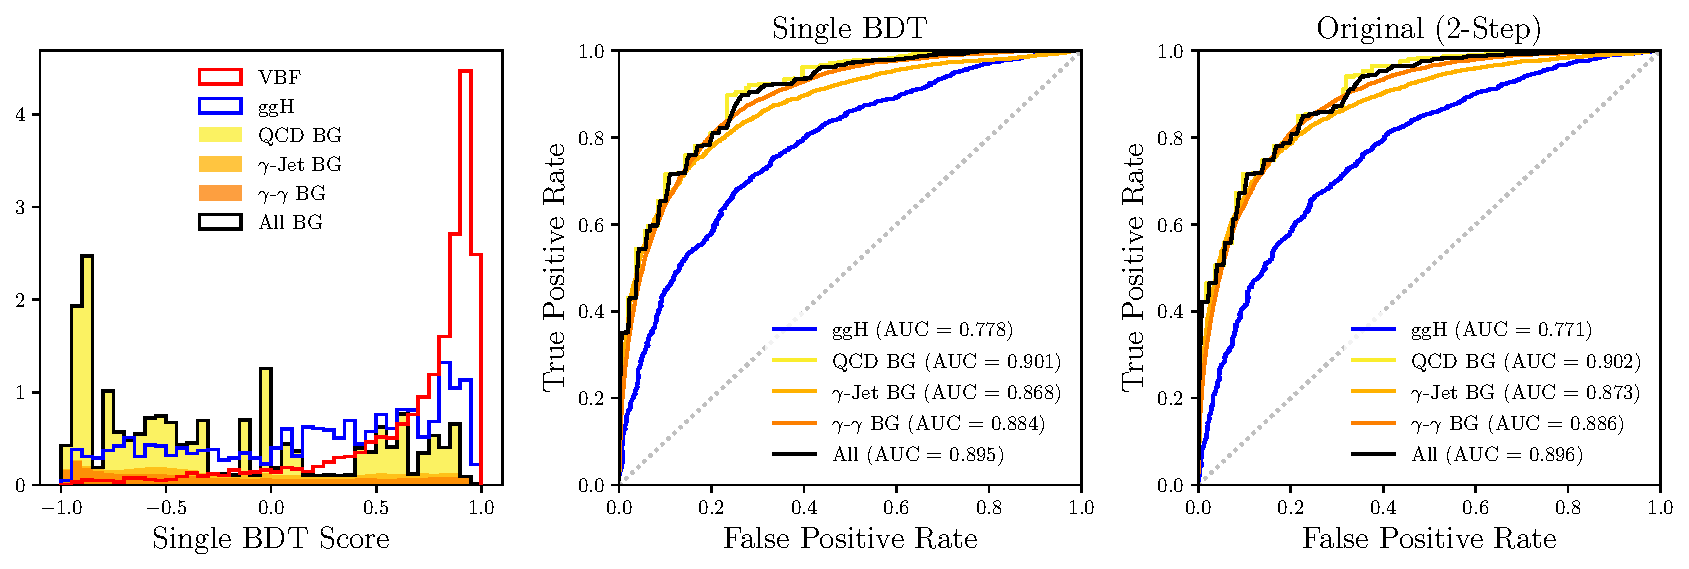
\includegraphics[width=0.99\textwidth]{figures/event_selection/dijet_BDT_PS_unw.pdf}
    \caption{Single BDT performance and comparison to the two step approach. Distributions of the single BDT score are shown on the left and are all normalised to unity with solid red corresponding to VBF, blue line to ggH, and black line to SM backgrounds. The SM background distribution is shown as a stacked histogram. Corresponding ROC curves for the single BDT (centre) and original approach (right) are shown with colours denoting the same samples as the histogram.}
    \label{fig:event_categorisation:single_BDT}
\end{figure}

















%=================================================
%---Dense CNN tag
%=================================================
\section[DCNN VBF Tag]{VBF Tag with a Dense Convolutional Neural Network}
In the BDT-based tag the ggH separation power is much lower than the SM background samples. 
This is a challenging problem to solve when equipped with only kinematic variables. Jet structure variables should offer important extra information.

Rather than using hand-engineered jet structure features, this problem is approached by formulating jet structure as an image and then training a dense convolutional neural network.
The model will form many discriminating features as part of the learning process, some hopefully more sophisticated  and more powerful than common engineered features. 

This section will describe the construction of these images, and the model built to process them in detail. The optimisation techniques for selecting the model structure are described, and the features the model has learned will be explored using a collection of techniques. After this the model will be validated with particular emphasis on how it is affected by the quality of QCD event modelling. 





\subsection{Jet Images}
The properties of a jet's constituent particles can provide important information about the originating parton. 
An image is a natural way of representing this information, with the spatial distribution represented by the arrangement of pixel values and the channels of the image representing properties such as charged particle $p_{T}$ deposition in the pixel region. 

\subsubsection{Formulation}
The image formulation used in this thesis (Figure \ref{fig:event_categorisation:jet_image}) is inspired by \cite{JetsInColour}, and uses two three-channel jet images (corresponding to the leading and subleading jets) stacked in the channels' dimension to produce a $n\times{}n\times{}6$ dijet image.
The three channels are the following: $p_T$ deposition of charged PF candidates, $p_T$ deposition of neutral PF candidates, and PF candidate multiplicity.
The space that the pixels correspond to is the space of particle displacements in pseudorapidity and azimuthal angle from the jet axis $(\Delta\eta,\Delta\phi)$,
\begin{equation}
    \begin{split}
        \Delta\eta =& \eta_{p} - \eta_{j} \\ 
        \Delta\phi =& \phi_{p} - \phi_{j} \\
    \end{split}
    \label{eq:event_categorisation:pixel_coords}
\end{equation}
where subscript $p$ denotes a constituent particle and $j$ denotes the jet. 
The pixels themselves are not a rectilinear grid in $(\Delta\eta,\Delta\phi)$, but are evenly-spaced in the polar coordinates 
\begin{equation}
    \begin{split}
        \Delta{R} =& \sqrt{\Delta\eta^2 + \Delta\phi^2} \\
        \varphi   =& \mathrm{atan2}(\Delta\phi,\Delta\eta) \\
    \end{split}
    \label{eq:event_categorisation:pixel_coords}
\end{equation}
These have been rotated by half a pixel in $\varphi$ so that the $(\Delta\eta,\Delta\phi)$ axes line up with the centres of a row of pixels rather than the boundary between them. 
Finally, the images are normalised such that the sum of the $p_T$-based channels equal one, and the sum of the individual multiplicity channels equal one. 
All of the images in this thesis will have the same form and are always centred on the jet axis.

\begin{figure}[h!]
    \centering
    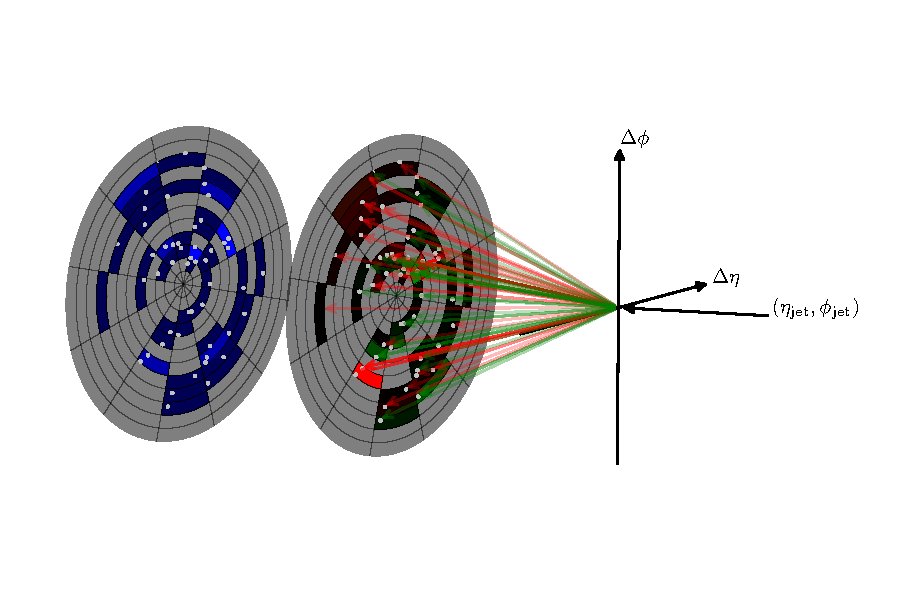
\includegraphics[width=0.9\textwidth]{figures/event_selection/jet_diagram_RGB.pdf}
    \begin{center}
        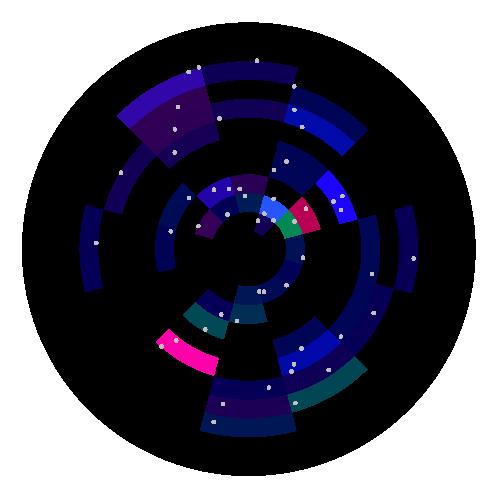
\includegraphics[width=0.45\textwidth]{figures/event_selection/full_image_polar.pdf}
        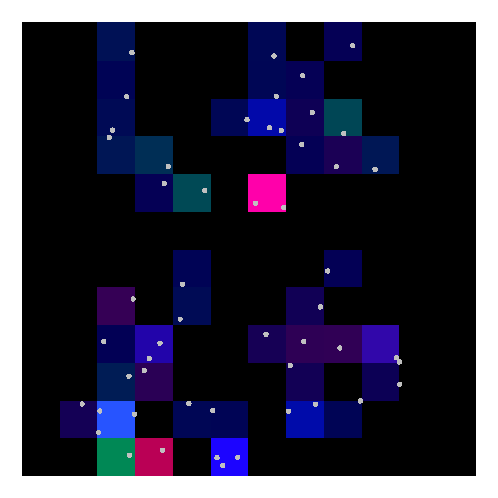
\includegraphics[width=0.45\textwidth]{figures/event_selection/full_image_rect.pdf}
    \end{center}
    \caption{Construction of single $12\times{}12$-pixel three-channel jet image (top). 
             Arrows correspond to individual jet constituents where red arrows are charged, green are neutral and the opacity of the arrows corresponds to candidate $p_{T}$.
             The multiplicity channel is drawn separately, and black pixels lightened so the charged and neutral channels can be seen clearly.
             The final image (bottom) shown in both $(\Delta\eta,\Delta\phi)$ coordinates (left) and the $(\Delta{R},\varphi)$ coordinates seen by the network (right).}
    \label{fig:event_categorisation:jet_image}
\end{figure}

%(Why this formulation: why polar images and why stack two jets?)
%(Translation invariance and cross-correlation between jets at low level)

This stacked dijet image formulation is used to facilitate finding correlations in structure between the two dijet jets. 
In this formulation it will happen at a lower level rather than constructing complex features on a per-jet basis and then comparing them. 
For example, this is needed for detecting the characteristic colour connection of VBF: if the jets are in opposite hemispheres the jet image will show the candidates to be pulled in opposite $\Delta\eta$ directions. 

Polar coordinate pixels are used to give finer segmentation at the centre of the jet and to make it easier for a DCNN to construct translation-invariant filters. Features will depend more on $(\Delta{R},\varphi)$ than $(\Delta\eta,\Delta\phi)$. 


\subsubsection{Image Dataset and Preprocessing}
These images are different in their formulation and behaviour compared to a typical image one finds in computer vision problems.
Firstly, they are sparse with only a fraction of the pixels ever non-zero in any one image. 
Secondly, assumptions about local correlations between pixels do not apply: two adjacent red pixels would mean two adjacent particles. Max pooling will simply pick the higher valued pixel during downsampling and information about the second particle will be lost. 
Thirdly, in the rectilinear image which is seen by the network (bottom right of Figure \ref{fig:event_categorisation:jet_image}) there is a periodic boundary condition where the top pixels wrap around to the bottom ones. When convolution operations are performed on these images the padding must be periodic in the vertical direction ($\varphi$ direction).

The dijet image distribution has a few notable features that originate from the structure of CMS. Outside the tracker acceptance there is no charge measurement and therefore the charged \pt channel may be all zero. The coarse structure of the forward detector regions also gives a change in image properties: here the images become constrained to a grid of dots. This can be see in the mean images shown in Figure \ref{fig:event_categorisation:mean_jet_images} where it manifests as a green grid in the mean of the image distributions (especially in VBF).

\begin{figure}[h!]

    \centering
    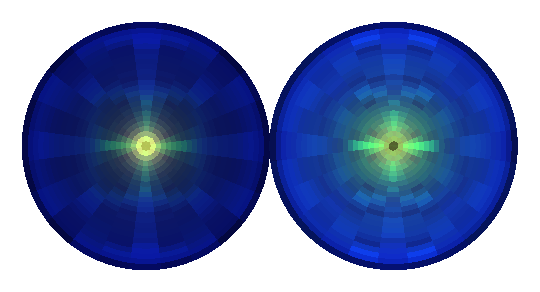
\includegraphics[width=0.49\textwidth]{figures/event_selection/mean_vbf_LPS_uw.pdf}
    \begin{center}
        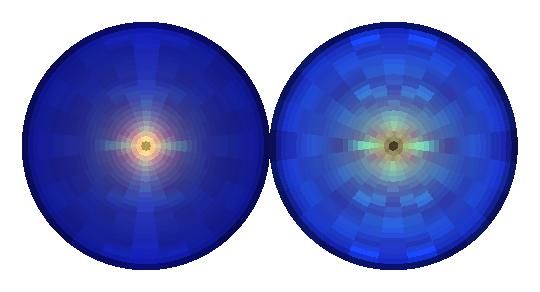
\includegraphics[width=0.49\textwidth]{figures/event_selection/mean_ggh_LPS_uw.pdf}
        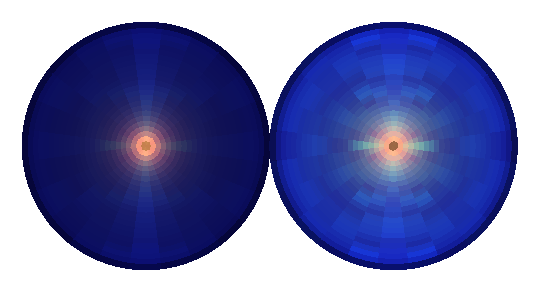
\includegraphics[width=0.49\textwidth]{figures/event_selection/mean_bkg_LPS_uw.pdf}
    \end{center}
    \caption{Mean dijet images for VBF events (top), gluon fusion events (bottom left) and Standard Model background processes (bottom right). In each dijet image the left hand image corresponds to the leading jet and the right corresponds to the subleading jet.}
    \label{fig:event_categorisation:mean_jet_images}
\end{figure}

Images are preprocessed before being input to the DCNN for both training and inference such that each feature (image pixel channel value) distribution has mean zero and standard deviation of one. 
This is achieved by subtracting the per-feature mean of the dataset and dividing by the per-feature standard deviation.
In this case the class-balanced mean and standard deviation are used where each class has equal weight. This is important for when the training is carried out over class-balanced minibatches.



\subsection{Dense CNN Model}

\subsubsection{Model Design}
The overall structure of the model can be considered to built from three main parts:
\begin{itemize}[noitemsep]
    \item \textbf{Convolutional section} for learning dijet substructure features from dijet images.
    \item \textbf{Merge section} for processing and integrating engineered kinematic features with learned features from the convolutional section.
    \item \textbf{Main discriminant} fully-connected layers for integrating all information and producing the class logits.
\end{itemize}

The \textbf{convolutional section} consists of a `spread layer' (SL) followed by three dense blocks (DB1, DB2, DB3) each of which are followed by transition units (TU1, TU2, TU3). All layer activation functions are leaky ReLUs to avoid the dying ReLU problem.

The spread layer is a depth-wise convolution layer that produces $N$-many feature maps for each channel where the filters do not mix the image channels. 
For each channel's associated feature maps half of them have their values evenly permuted in the vertical direction, this corresponds to a rotation by $\pi$ in the polar image.
The function of this layer is to spread-out the sparse image into a collection of feature maps that correspond to simple local spatial configurations of pixels such as radial or angular bands of deposition. 
The interleaved rotations of this layer's output feature maps allows for the comparison of pixels opposite each other around the jet axis much earlier in the network.  
This layer gives two hyperparameters to the model: the filter size and the number of features per input channel.

The dense blocks construct increasingly higher-level feature maps, and the transition units combine feature maps for feature reduction as well as downsampling with average pooling to avoid information loss associated with max pooling mentioned before.  
The structure of each of these parts is tuneable, and therefore gives another twelve hyperparameters to the model: three from each dense block and one from each transition unit. 

The \textbf{merge section} consists of a set of fully-connected layers with the first one after the initial input a different size to the others. This is then concatenated with the output of the convolutional part.
The function of this section is to embed the engineered features in a higher-dimensional space, form them into a vector the same size as the convolutional section output, and then combine them together with the jet structure features. This section has three hyperparameters: the size of the hidden layers, the number of layers, and the size of the first hidden layer relative to the others. 


The \textbf{main discriminant} consists of a sequence of fully-connected layers that take the full vector of concatenated features as input and produce three class logits which correspond to the VBF, ggH, and SM background process classes. 
These logits are then mapped to class probabilities by a softmax function. The VBF class probability is then used to define tag categories. 

In addition to the above, the formulation of the image can also be tuned like another hyperparameter to choose the most performant number of pixels. 



\subsubsection{Image Formulation and Network Architecture Search}
%intro
Choosing the specific network architecture is a complex and time-consuming problem as there are many hyperparameter choices to explore and model training can take as long as 24 hours.
To find an optimal model in the space of possible hyperparameter choices an optimisation scheme based on Bayesian optimisation is used. 


%procedure
As the training time is a severe bottleneck the hyperparameter space is sampled for trainings on the two-class subproblem of only VBF/ggH. 
The metric to be optimised for is the peak AUROC evaluated on the validation set during training, and each training can only take a maximum of 24 hours. 
This time requirement is to keep the model size and therefore training time to a practical level for use in a physics analysis.  
The optimisation is split into a series of steps targeting different parts of the hyperparameter space.
All of these optimisations were carried out using the Imperial College London Research Computing Service \cite{IC_HPC}.

First an approximate optimisation is carried out over all of the structure hyperparameters to ensure that the candidate model is not in a strongly suboptimal region to begin with. 
Next the choice of image channels and pixels is optimised to find the optimal image formulation. After this the spread unit, dense block and transition unit depth structure are optimised and then another optimisation is carried out for the filter sizes in the spread layer and dense blocks. Finally, the depth and size of the fully-connected layers of the merge unit and main discriminant are optimised. 

%result
The final optimised structure is as follows.
\begin{itemize}[noitemsep]
    \item Image: $24\times{24}$ pixels with charged \pt, neutral \pt, and multiplicity for each jet.
    \item SL: 16 features per channel with a filter size of $5\times{}5$.
    \item DB1: 3 layers with growth rate 20 and filter size $3\times{}3$.
    \item TU1: reduction factor of $0.59$.
    \item DB2: 6 layers with growth rate 10 and filter size $3\times{}3$.
    \item TU2: reduction factor of $0.95$.
    \item DB3: 16 layers with growth rate 4 and filter size $3\times{}3$.
    \item TU3: reduction factor of $0.5$.
    \item Merge: first layer size factor $1.5$, layer size 512, depth 2.
    \item Discriminant: layer size 512, depth 3.
\end{itemize}
The optimisation appears to have favoured more abstract and complex features later in the model where the field of view is larger. This is shown by the fact that much of the depth is introduced in DB3. 
There is also a strong feature reduction in TU3 that strongly curtails model complexity. High-dimensional output from the convolutional section leads to a large increase in parameters due to the fully-connected layer immediately after it. 




\subsubsection{Regularisation}
%Intro
The DCNN model is regularised with a single $L_2$ regulariser term for the convolutional section, dropout, and gradient clipping.

%L2 regularization
$L_2$ regularisation encourages the learning of smoother features in the convolutional section and was found in optimisation studies to give better performance than $L_1$ or $L_1 + L_2$. 
In the $L_1 + L_2$ optimisation the $L_1$ term became very small and effectively converged to the $L_2$ result.
A three-dimensional Bayesian optimisation was carried out to tune the final $L_2$ hyperparameters for the convolution, merge and main discriminant sections.
This optimisation showed that very small values are preferred in the non-convolutional sections, and they were therefore set to zero. 
The use of $L_2$ regularisation in the convolutional section will encourage smoother features. This may stop the model memorising particular configurations of pixels and prevent overfitting. 
It is desirable that the representation learned by the model is spread-out in the neurons as this leads to robustness and better generalisation \cite{DeepMindDeletion}.
This is another effect of $L_2$ regularisation.

%Dropout
Dropout is used in all sections, but the dropout in the convolutional section is different to standard dropout. 
In the convolutional section spatial dropout is used where entire feature maps are dropped rather than individual neurons. 
This stops the model from getting over-reliant over particular features and is another way of encouraging a more spread-out representation. 


%Gradient clipping
Gradient clipping is particularly crucial to keep training updates stable in this model. 
The scheme limits the maximum size of parameter updates during stochastic gradient descent by clipping the gradients to some maximum value. 
Specifically this is done by calculating the global $L_2$ norm of the gradient vector in the parameter space and scaling the gradient vector back if it is over the maximum value.  

This is necessary when the loss surface as a function of the model parameters has cliff-like regions. If the gradient is evaluated at the cliff face the gradient may be very large which will lead to a very large parameter update kicking the parameters of the model far from the point it was evaluated at. Gradient clipping will stop this from happening by keeping the parameter update small and allowing the parameters of the model to settle at the bottom of the cliff. These cliff-like regions are common when dealing with sparse inputs where most values are zero, therefore this is most likely a consequence of the dijet image sparsity. 



\subsubsection{Loss}
The loss function encodes an opinion of what constitutes good model performance and it is here that one can define the cost of particular sorts of misclassification over others. 
There are two components to this: inter-class costs and intra-class costs. 

\textbf{Inter-class} cost defines the relative priority of misclassification between the classes. 
This was attempted in a less formal manner in the BDT-based model when ggH was left out of the combined BDT training. 
This would be equivalent to setting the misclassification cost for the ggH events to zero. 

For the DCNN-based model a cost-sensitive version of cross entropy developed in \cite{CostSensitivity} is used,
\begin{equation}
    L_i = -\log\left(\frac{\xi_{pp}e^{o^{i}_{p}}}{\sum_{j=0}^{2}\xi_{pj}e^{o^{i}_{j}}}\right)
\end{equation} 
where $i$ enumerates the events of the minibatch, $o_j$ is the logit of class $j$, $p$ is the true class index of the event, and $\xi$ is the cost matrix which encodes misclassification costs.
The cost matrix has the following definition,
\begin{equation}
    \xi = \begin{pmatrix}
        c_{\mathrm{BG}} & c_{\mathrm{BG}/\mathrm{ggH}} & c_{\mathrm{BG}/\mathrm{VBF}} \\
        c_{\mathrm{BG}/\mathrm{ggH}} & c_{\mathrm{ggH}} & c_{\mathrm{ggH}/\mathrm{VBF}} \\
        c_{\mathrm{BG}/\mathrm{VBF}} & c_{\mathrm{ggH}/\mathrm{VBF}} & c_{\mathrm{VBF}} \\
    \end{pmatrix}
\end{equation}
where each element $c$ is a real number belonging to the interval $(0,1]$ on the diagonal and $[0,1]$ off-diagonal. 
This was selected to be symmetric to simplify the cost optimisation problem.
If all the elements are set to one this is equivalent to ordinary cost-insensitive cross entropy. 

When training the model $c_{\mathrm{BG}/\mathrm{ggH}}$ is set to zero as this type of misclassification does not matter at all in the VBF tag. 
The training should not compromise on other types of misclassification to improve it. 
This leads to the largest performance increase in VBF discrimination and is crucial to being able to treat this as a three-class problem.
The diagonal values are all set to one, tuning this was found to make little difference. These entries are equivalent to setting the general cost of misclassifying a class.
The cost $c_{\mathrm{BG}/\mathrm{VBF}}$ is kept at one as this type of discrimination is the primary objective of the model. 
Finally, $c_{\mathrm{ggH}/\mathrm{VBF}}$ was tuned to maximise VBF/ggH discrimination while keeping VBF/BG discrimination at or above the level of the BDT-based model. This was found to be $0.5$.

\textbf{Intra-class} costs are introduced by weighting events in each minibatch depending on their event weight and their class.  
Within each class in the minibatch each event is given a weight in proportion to its event weight scaled to belong to an interval $[1,a]$ where $a$ is a positive real number greater than one. 
If this scaling is not used the difference in weight between events can be multiple orders of magnitude leading to instability and underperformance. 
The total weight for each class is then scaled to be equal to mitigate the effects of class imbalance. 

The loss over the entire minibatch is expressed as a weighted sum of events,
\begin{equation}
    L = \frac{1}{\sum_{j=0}^{N-1}w_{j}}\sum_{i=0}^{N-1}w_{i}L_{i}
\end{equation} 
where $N$ is the number of events in the minibatch, and $w_i$ is the weight of event $i$.
This is the final loss that is minimised by the optimiser during training. 



\subsubsection{Training Process}
%intro
%Training is done in two steps: image only and then the rest. This is why...
The training process consists of two steps: first the convolutional part is trained on its own with two fully-connected layers, then the convolutional layer parameters are frozen and the full model is trained with the engineered features. This approach is used because it was found that when the convolutional section is trained simultaneously with the rest of the network, the training is less stable and the model under performs.

%Convolutional section training
The objective of the convolutional section training is to develop the learned features that will be used in the full model. 
This is targeting VBF/ggH discrimination, therefore training is treated as a two-class problem with just the ggH and VBF samples.  

This runs over 150000 batches of 900 events with event weights equal to one. Each batch is class-balanced and contains 450 events from each of ggH and VBF.  
During the training the data are augmented by randomly reflecting the images in the $\Delta\eta$ and $\Delta\phi$ directions to improve generalisation. 

The optimisation algorithm used is Adam with Nesterov momentum (Nadam) with learning rate $0.001$ and the loss used is cross entropy. 
Nadam was found to be the most performant in contrast to the CNN literature where SGD with Nesterov momentum is consistently better. 
This is likely due to adaptive learning rate algorithms such as Adam having parameter-specific learning rates that are increased if the parameter does not change much. 
This makes them better at handling sparse network inputs which can result some parameters of the network not being updated as often as others. 



%Integration training
The trained convolutional model then has its parameters frozen, and the fully-connected layers after the convolutional section (after TU3) are removed. 
The output of TU3 will be the learned features produced in the first training step, they are then concatenated with the `spread-out' engineered features of the merge section.
Another training is then performed over the full training set to train the merge section and the final discriminant. 

This training runs over 100000 batches of 900 events with scaled event weights as described in the loss subsection. 
Each batch is again class-balanced, but this time it has 300 events from the three classes: VBF, ggH, and SM background. 
The optimisation algorithm is Nadam with the same learning rate and the loss is the cost-sensitive cross entropy described previously. 














\subsection{Model Performance}
%Image only performance (Text and figure)
To determine how the learned features contribute to VBF/ggH discrimination performance the image-only network (stage one of the training) may be compared to the single-step BDT model.
This performance is examined on the same test set with both the loose and full VBF preselections.
On the loose preselection the image-only network achieves an AUROC of $0.800$ which is already better than the $0.796$ of the BDT (Table \ref{tab:event_categorisation:auroc_table}) 
However, upon moving to the full PS the image-only performance drops below the BDT. The score distribution and the associated ROC curve for the image-only model are shown in Figure \ref{fig:event_categorisation:image_only_DCNN}. This drop is possibly due to the more stringent \pt cuts removing gluon jets which have a softer \pt spectrum.
\begin{figure}[h!]
    \centering
    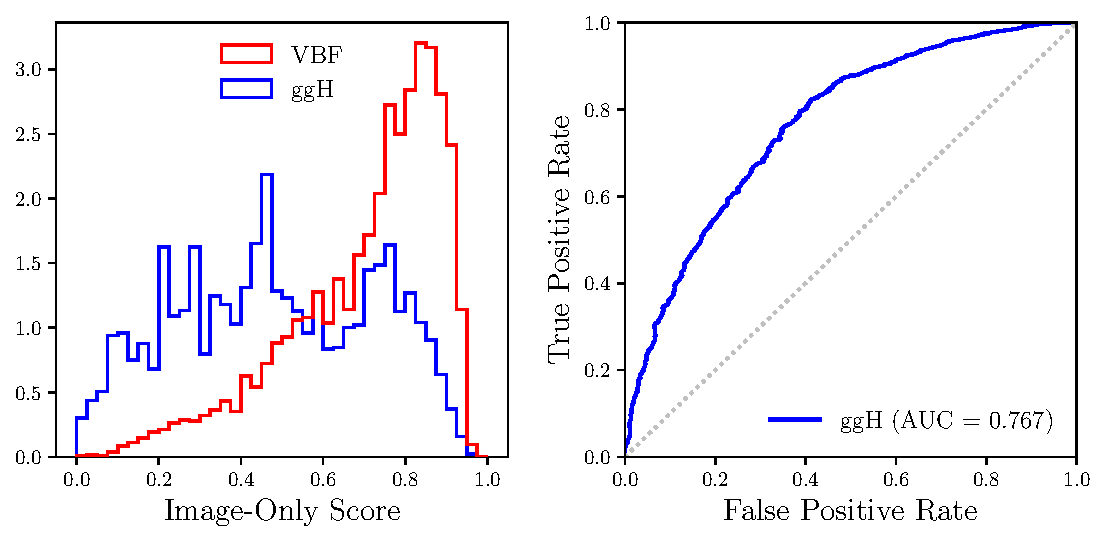
\includegraphics[width=0.9\textwidth]{figures/event_selection/imgonly_DCNN_PS.pdf}
    \caption{VBF/ggH discrimination performance for the image-only model with the full VBF preselection. The score distribution for VBF (red) and ggH (blue) is shown on the left. The associated ROC curve measuring VBF/ggH discrimination power is shown on the right.}
    \label{fig:event_categorisation:image_only_DCNN}
\end{figure}

%Full model performance 
The full model includes the same set of kinematic variables as the BDT and has been trained with the tuned costs over all of the backgrounds (stage two of the training).
This model brings a substantial improvement in the VBF/ggH discrimination, especially with the full preselection. 
For the other background samples the performance is similar with the DCNN AUROCs being slightly higher. 
This information is summarised in Table \ref{tab:event_categorisation:auroc_table} and the score distribution with the associated ROC curves are shown in Figure \ref{fig:event_categorisation:perf_full_DCNN}.
\begin{table}[h!]
    \centering
    \renewcommand{\arraystretch}{1.3}
    \begin{tabular}{l|cccc}
        \thickhline
        & \multicolumn{2}{c}{Full PS} & \multicolumn{2}{c}{Loose PS} \\ 
        Sample & BDT & DCNN & BDT & DCNN \\
        \hline
        ggH             & 0.778 & 0.837 & 0.796 & 0.845\\
        QCD             & 0.901 & 0.907 & 0.892 & 0.885\\
        $\gamma$-jet    & 0.868 & 0.870 & 0.869 & 0.882\\
        $\gamma\gamma$  & 0.884 & 0.891 & 0.870 & 0.881\\
        All             & 0.895 & 0.901 & 0.883 & 0.884\\
        \thickhline
    \end{tabular}
    \caption{Comparison table for BDT/DCNN AUROCs with full and loose preselections broken down by background sample.}
    \label{tab:event_categorisation:auroc_table}
\end{table}
\begin{figure}[h!]
    \centering
    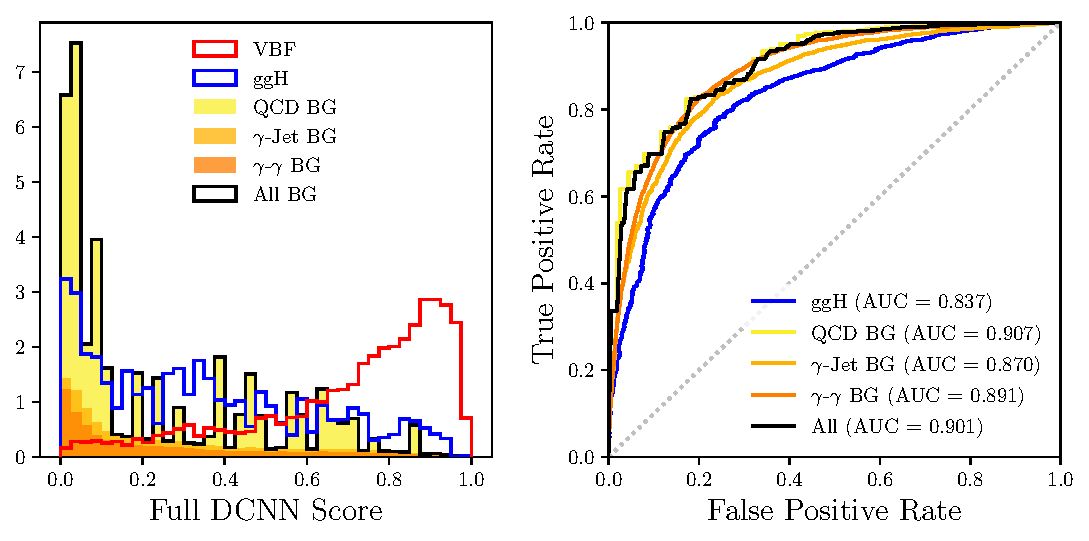
\includegraphics[width=0.9\textwidth]{figures/event_selection/full_DCNN_PS.pdf}
    \caption{Discrimination performance for all of the background samples with the full model and the full VBF preselection.
             Score distributions (left) are shown as stacked histograms for the SM background, a blue line histogram for ggH, and a red line histogram for VBF. 
             Associated ROC curves (left) are shown in the same colours for each sample, with all background together shown in black.}
    \label{fig:event_categorisation:perf_full_DCNN}
\end{figure}

In conclusion, the DCNN-based model demonstrates a strong improvement over the BDT-based model in VBF/ggH discrimination and the learned features alone are strongly discriminating. 












\subsection{Categorisation and Tag Performance}
To determine how the higher model performance of the DCNN translates into the VBF tagging and categorisation itself, the category boundaries are re-evaluated. 
This uses the same procedure as before for the boundary optimisation itself and the number of categories. 
The optimal number of categories for the DCNN-based VBF tag is found to be three.
Approximate studies of the three VBF categories, their boundaries and their estimated performance is shown in Figure \ref{fig:event_categorisation:DCNN_mass_fits} and Table \ref{tab:event_selection:DCNN_cats}.
\begin{table}[h!]
    \centering
    \renewcommand{\arraystretch}{1.3}
    \begin{tabular}{ l | c c c c c }
        \thickhline
        Category & Score Range & $\sigma_{\mathrm{eff}}$ & AMS & $B_{\mathrm{ggH}}/(S+B_{\mathrm{ggH}})$ & $S/(S+B)$ \\
        \hline
        VBF 0 & $[1, 0.856)$     & 1.5 &  2.13 & 0.10 & 0.37 \\
        VBF 1 & $[0.856, 0.704)$ & 2.0 &  1.15  & 0.27 & 0.11 \\
        VBF 2 & $[0.704, 0.495)$ & 2.0 &  0.60 & 0.46 & 0.04 \\
        \thickhline
    \end{tabular}
    \caption{Estimated category attributes for the DCNN-based VBF tag.}
    \label{tab:event_selection:DCNN_cats}
\end{table}
\begin{figure}[h!]
    \centering
    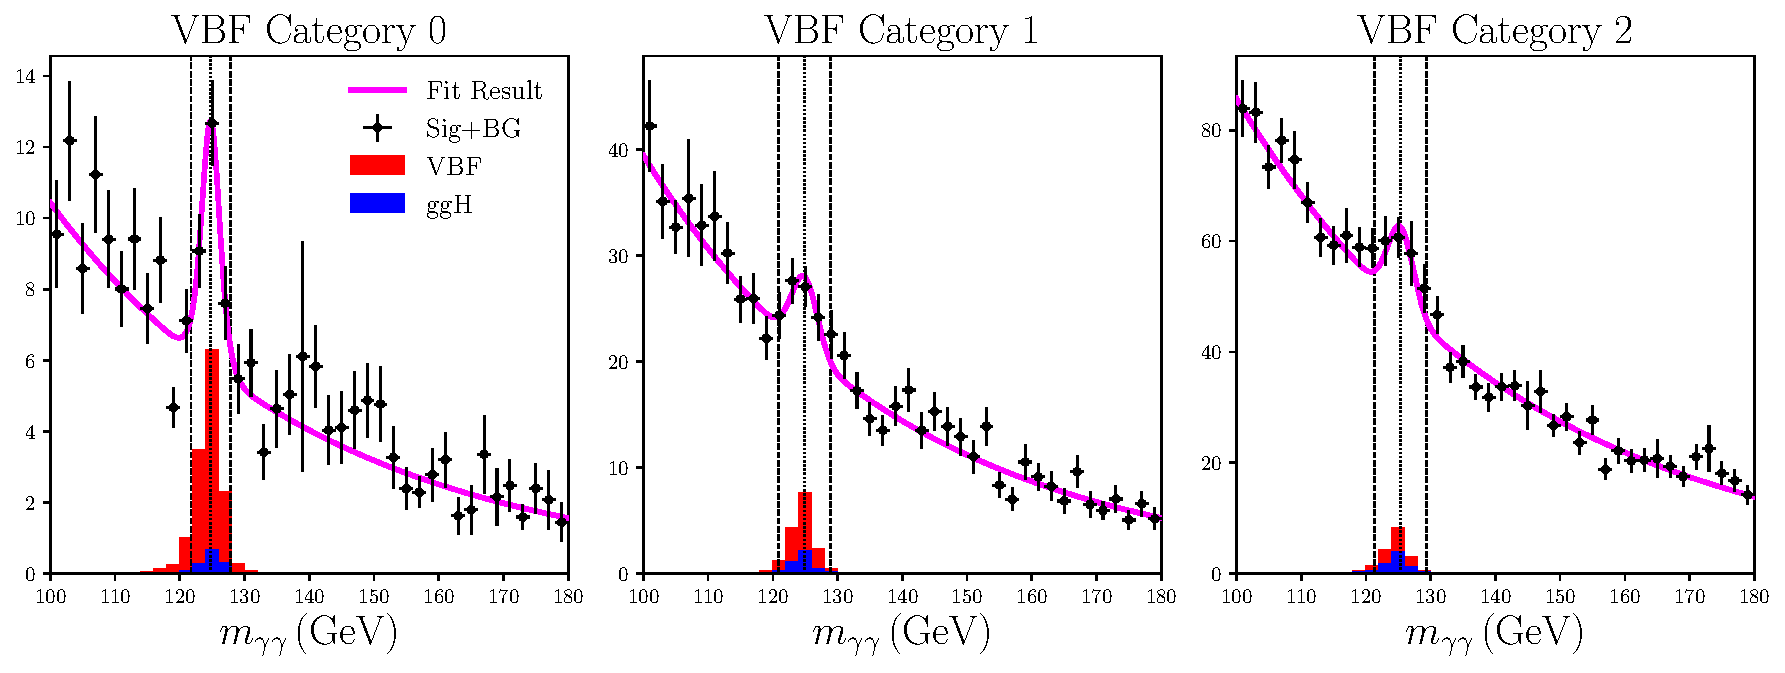
\includegraphics[width=1.0\textwidth]{figures/event_selection/DCNN_mass_fits.pdf}
    \caption{Mass distributions and fits for the three optimised DCNN-based tag categories.}
    \label{fig:event_categorisation:DCNN_mass_fits}
\end{figure}

The proper measurement of these category performances requires the full machinery of the signal and background modelling, and the final fits of Chapter \ref{chap:statistical}.
These studies show a reduction in the ggH contamination of VBF 0, but the other categories are approximately unchanged. 
This demonstrates the challenge of improving ggH discrimination as it needs to be traded off against overall background rejection performance, and as a corollary; statistical significance.









\subsection{Model Interpretation}
A collection of techniques can be used to determine what sort of features the convolutional section is learning to form.
This section will explore three: feature visualisation with synthetic images generated to maximally activate part of the network, real images that achieve the same thing, and direct inspection of the frontmost filters (filters of the spread layer).



\subsubsection{Feature Visualisation}
The technique of feature visualisation uses optimisation and differentiability of neural networks to interpret their inner workings, particularly CNNs \cite{FeatureVis}. A famous example of this process is inceptionism and the so-called `deep dream' images \cite{Inceptionism}. The network is in effect forced to `hallucinate' by creating a feedback loop between its visual input and neural activations that iteratively alters the visual input to maximise the activation.

The approach used in this thesis is based on SGD with momentum and no regularisation or other conditions. 
The process begins with an initial image tensor, $x_{ijk}$, with small random positive values, and a momentum tensor, $v_{ijk}$, of the same size initialised to zero.
The loss in this case will be a single output neuron $o_{l}$. The image is then altered as follows:
\begin{equation}
    \begin{split}
        v_{ijk} &= \mu{}v_{ijk} + \alpha\frac{\partial{o_{l}}}{\partial{x_{ijk}}} \\
        x_{ijk} &= x_{ijk} + v_{ijk}
    \end{split}
\end{equation} 
where the partial derivative has been computed with backpropagation, and $\alpha$ is the learning rate. Negative pixel values are set to zero and the image is normalised as described in the image formulation section before the next iteration. This continues for 1000 iterations with the learning rate reduced by a factor of $0.75$ every 100 iterations. 
The end results of this for the VBF and ggH logits of the image only network are shown in Figure \ref{fig:event_categorisation:feature_vis_vbf_ggh}.
\begin{figure}[h!]
    \centering
    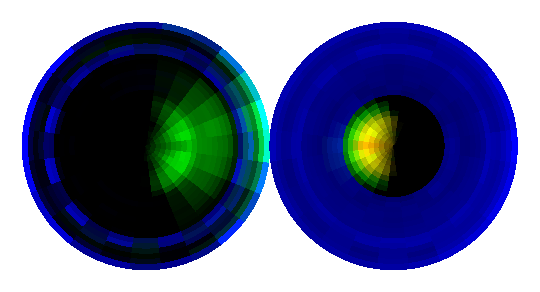
\includegraphics[width=0.85\textwidth]{figures/event_selection/norm_logits1.pdf}
    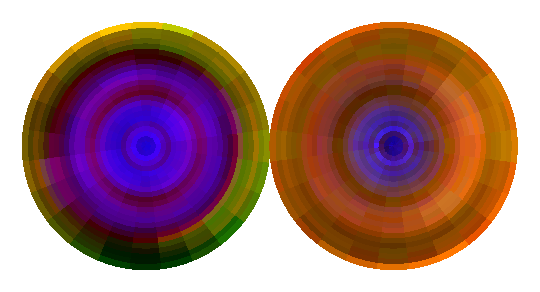
\includegraphics[width=0.85\textwidth]{figures/event_selection/norm_logits0.pdf}
    \caption{Generated images for feature visualisation which maximally activate the output neuron: VBF (top) and ggH (bottom).}
    \label{fig:event_categorisation:feature_vis_vbf_ggh}
\end{figure}

These images show a clear difference in each class, and some interesting physical features. However, it should be noted that these will be somewhat unphysical as the optimisation will try to pack as much evidence for the target class in to the image as possible with no constraints on what is sensible. For example, if one takes a network such as inception and optimises for the dog class it will produce an image of a carpet of deformed dogs as the optimisation tries to include as many dog features as possible. 


The VBF image shows clear signs of colour connection where the jet constituents are pulled in opposite $\Delta\eta$ directions. This causes asymmetry in the jet image where there are more non-zero pixels on one half and the leading and subleading images have this asymmetry in opposite directions.
They are also more collimated with more \pt  deposition in the jet core as expected for quark jets. This can be observed as more colour at the centre of the image and more empty pixels around the outside. The dominance of neural \pt deposition (green) and discrete rings of multiplicity (blue) indicate that the model is forming features that detect jets in the forward regions by detector coarseness and lack of charge. 

In the ggH image a more circular structure can be seen with a larger proportion of charged deposition over a larger area. This is in line with the expectation that gluon jets are less collimated and higher multiplicity. The rings line up with the gaps in the coarse forward structure, this suggests that the model is learning to detect whether the jets are in the tracker acceptance. 


\subsubsection{Pseudorapidity Inference}
The structure of the feature visualisation images suggest that the model has learned to reconstruct a coarse estimate of the pseudorapidity properties of the jet: whether the jets are in the coarse forward regions or not. 
To test this hypothesis the second step of the training is run again with the leading and subleading jet pseudorapidities included in the engineered features. If there is no change in performance this would suggest that the model already has access to this information via the image input. This training shows no performance increase with the AUROCs of the two models being almost identical. This leads us to conclude that the network does indeed reconstruct this information or the information is not useful.

However, training a single BDT model with the pseudorapidities shows a small performance increase in discrimination power. This suggests that only a small portion of the DCNN performance gain comes from inferring the pseudorapidity. 


\subsubsection{Maximally-Activating Images}
To get a better idea of what sort of physically sensible features are favoured by the network, and whether the conclusions about the feature visualisation are true, real event images are inspected that are maximally activating. 
A selection is applied on the leading jet so that it is in the tracker acceptance and the charged-\pt  channel is present. The most activating image without this requirement shows two very forward jets with coarse structure.  The two maximally activating images for the VBF and ggH classes are shown in Figure \ref{fig:event_categorisation:maxact_vis_vbf_ggh}.
\begin{figure}[h!]
    \centering
    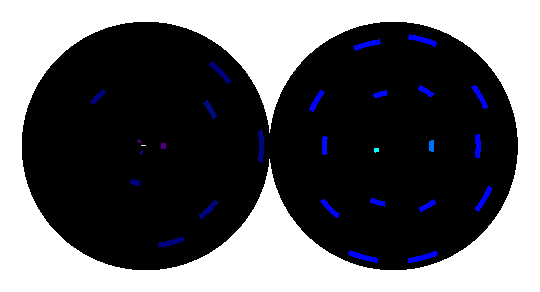
\includegraphics[width=0.85\textwidth]{figures/event_selection/max_img_vbf_tkr_cut_logits_normtype1.pdf}
    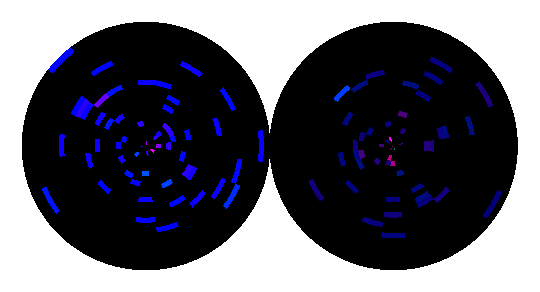
\includegraphics[width=0.85\textwidth]{figures/event_selection/max_img_ggh_tkr_cut_logits_normtype1.pdf}
    \caption{Real images that maximally activate the class logits. 
             The top image is the maximally-activating VBF image, and the bottom is the maximally-activating ggH image. }
    \label{fig:event_categorisation:maxact_vis_vbf_ggh}
\end{figure}

The max-activating images for ggH and VBF resemble the feature visualisations with SGD. 
The VBF image is collimated, with a spread in one $\Delta\eta$ direction in the leading jet and the opposite in the subleading. 
This effect is easier to see in the leading jet, but is also present in the subleading image where there is one bright pixel to one side.
The effect of the coarse forward structure of CMS on the subleading jet image can also be observed. 
The ggH is far higher in multiplicity, much less collimated and more circular. This is in line with the image from feature visualisation. 


\subsubsection{Front Filters and Low-level Features}
The lowest-level features that the network constructs are at the spread layer. 
This layer can be interpreted as forming local arrangements of pixels into more spread-out non-sparse feature maps. 
These convolution filters are shown in Figure \ref{fig:event_categorisation:front_filters}.

\begin{figure}[h!]
    \begin{center}
        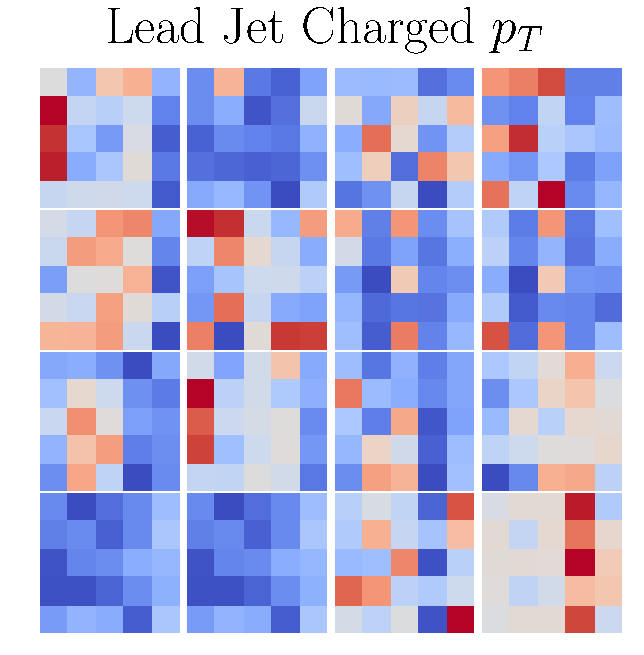
\includegraphics[width=0.32\textwidth]{figures/event_selection/front_filters_channel_0.pdf}
        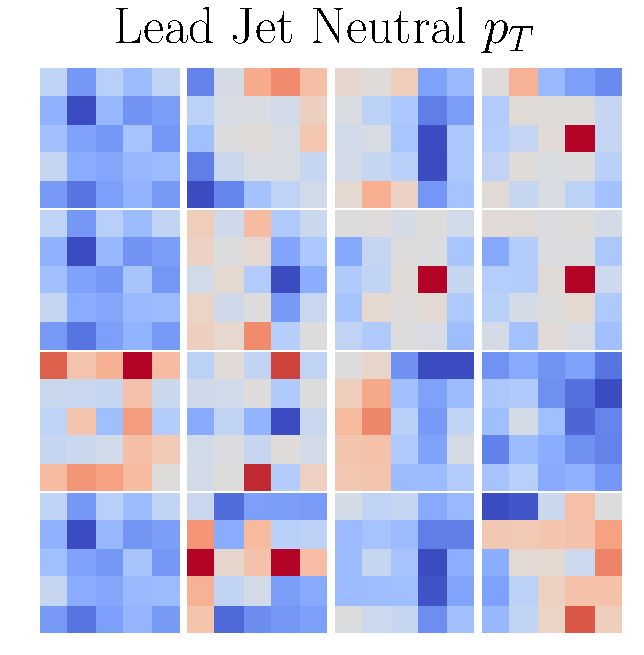
\includegraphics[width=0.32\textwidth]{figures/event_selection/front_filters_channel_1.pdf}
        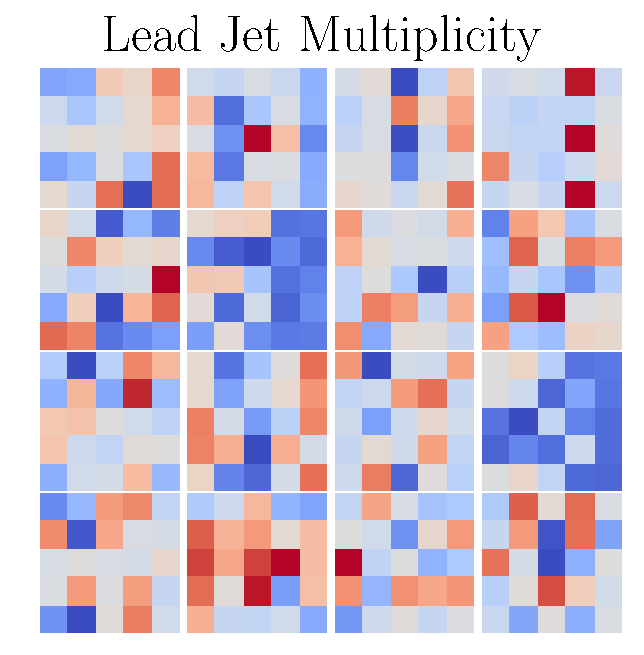
\includegraphics[width=0.32\textwidth]{figures/event_selection/front_filters_channel_2.pdf}
    \end{center}
    \begin{center}
        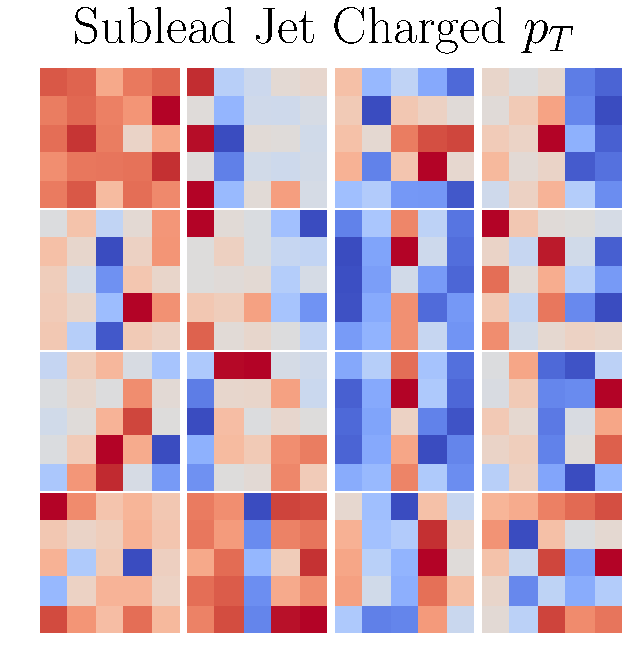
\includegraphics[width=0.32\textwidth]{figures/event_selection/front_filters_channel_3.pdf}
        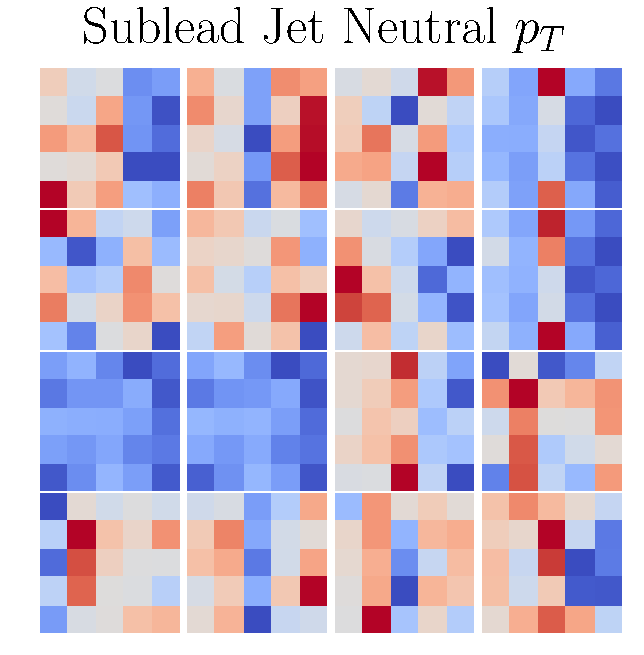
\includegraphics[width=0.32\textwidth]{figures/event_selection/front_filters_channel_4.pdf}
        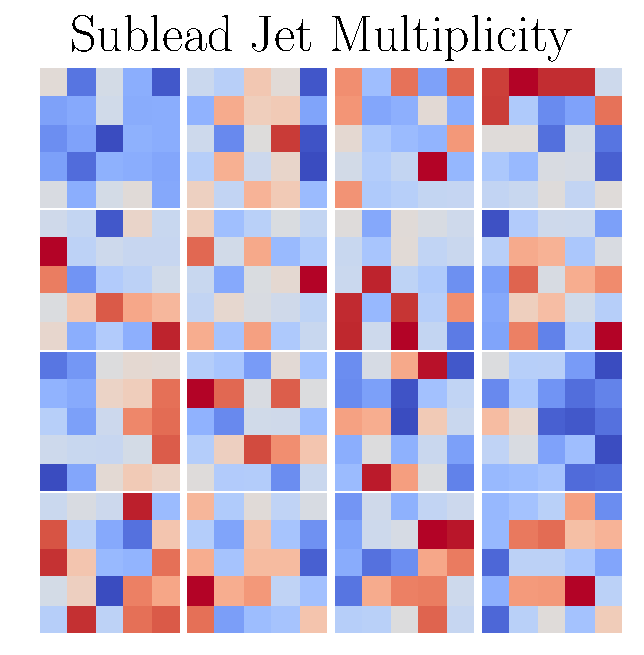
\includegraphics[width=0.32\textwidth]{figures/event_selection/front_filters_channel_5.pdf}
    \end{center}
    \caption{Front filters of the network grouped by the six image channels. Positive weight values are darker red and more negative values are darker blue, weights close to zero are shown as white. The vertical direction in the filters corresponds to $\varphi$ and the horizontal direction corresponds to $\Delta{R}$.}
    \label{fig:event_categorisation:front_filters}
\end{figure}

The front filters have a coarse and noisy appearance. This would be a sign of inappropriate training conditions in a CNN with normal images: either the learning rate is too high or the model requires regularisation. 
In this case the noisiness could be intrinsic to the dijet image problem because the images are sparse and are less smooth. Training without event weights, with large batches and a lower learning rate produced smoother filters and better generalisation performance.  

The filters themselves detect radial and angular bands of pixels, this corresponds to horizontal and vertical stripes in the filter. 
There are also filters that detect separated stripes of pixels these are two positive (red) stripes with a negative stripe (blue) in between. This behaves like an edge detection filter. 
Finally, there are filters where there is a single large-value weight offset from the centre of the filter. This appears to perform a small angular or radial shift in the jet image. 
Examples are shown in Figure \ref{fig:event_categorisation:filter_action}.
\begin{figure}[h!]
    \begin{center}
        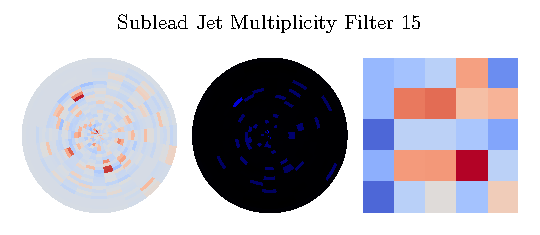
\includegraphics[width=0.49\textwidth]{figures/event_selection/ggh_firstconv_5_15.pdf}
        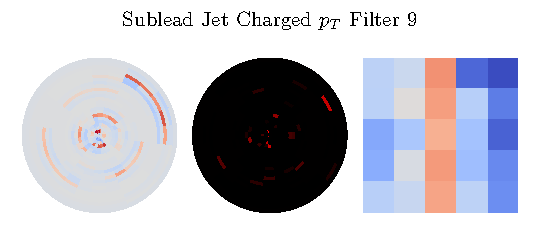
\includegraphics[width=0.49\textwidth]{figures/event_selection/ggh_firstconv_3_9.pdf}
    \end{center}
    \begin{center}
        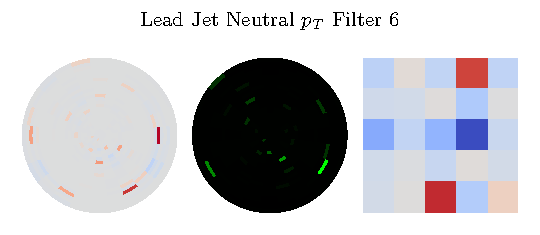
\includegraphics[width=0.49\textwidth]{figures/event_selection/ggh_firstconv_1_6.pdf}
        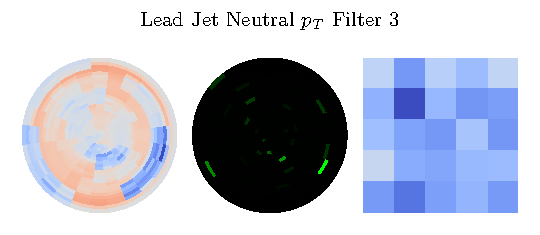
\includegraphics[width=0.49\textwidth]{figures/event_selection/ggh_firstconv_1_3.pdf}
    \end{center}
    \begin{center}
        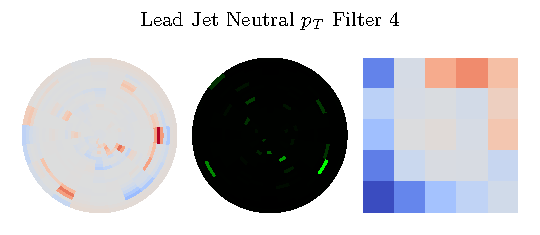
\includegraphics[width=0.49\textwidth]{figures/event_selection/ggh_firstconv_1_4.pdf}
        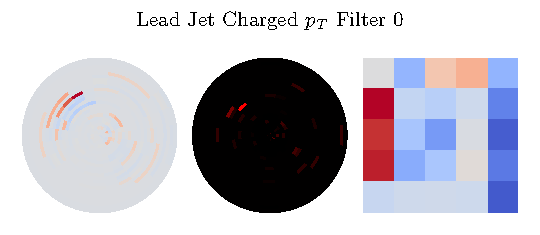
\includegraphics[width=0.49\textwidth]{figures/event_selection/ggh_firstconv_0_0.pdf}
    \end{center}
    \caption{The effect of selected filters. Each subplot shows the effect of the filter and subsequent neural activation (left), the original preprocessed image (centre) and the filter (right).
             Clockwise starting from top left the filters are: radial gap detector, angular band smearer, general smearer, angular smear with gap in front, radial and angular smearer with shifts, double shifter.}
    \label{fig:event_categorisation:filter_action}
\end{figure}



\subsubsection{Conclusion}
It has been shown that the network is capable of constructing sophisticated and physically relevant features of dijet substructure from the input images. 
It is learning to infer information about jet pseudorapidity, but this accounts for only a small portion of the performance increase. 
Furthermore, these studies show that feature visualisation and max-activation images are powerful techniques. 
These can be applied to any part of the network to extract information about its behaviour.  











\subsection{Validation}
The DCNN-based model may be particularly vulnerable to disagreement between simulation and data. The underlying QCD processes of the underlying event, parton showering, and hadronization are challenging to model and this may adversely affect the application of this model to real data. To determine whether this is the case the model is validated in the \Zee control region and with QCD modelling variations described previously with special attention given to how the performance of the image-only model changes.
The \Zee data/simulation disagreement will be investigated with a specially trained network. 

\subsubsection{\Zee Control Region}
First the simulation/data agreement of the network score is evaluated for both the image-only and the full DCNNs (Figure \ref{fig:event_categorisation:int_score_zee}). 
\begin{figure}[h!]
    \begin{center}
        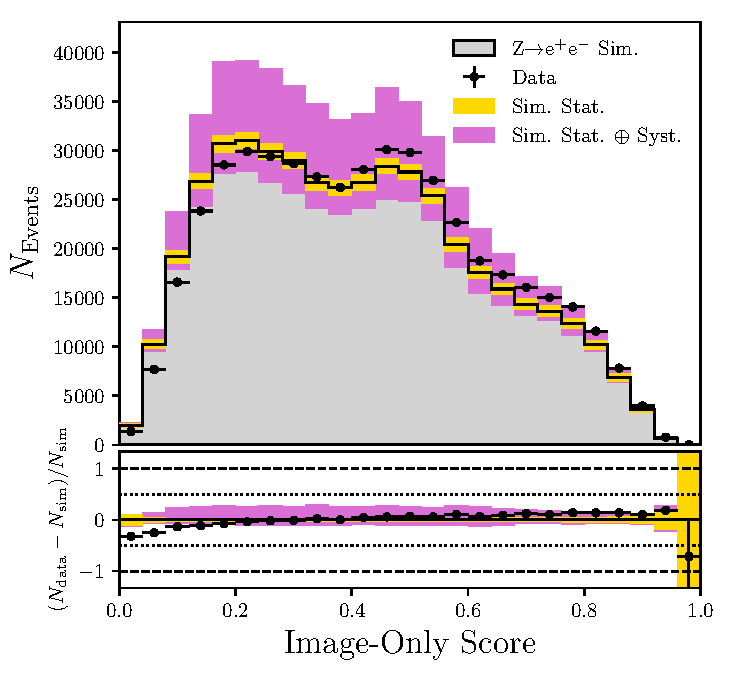
\includegraphics[width=0.49\textwidth]{figures/event_selection/img_score_zee_LPS.pdf}
        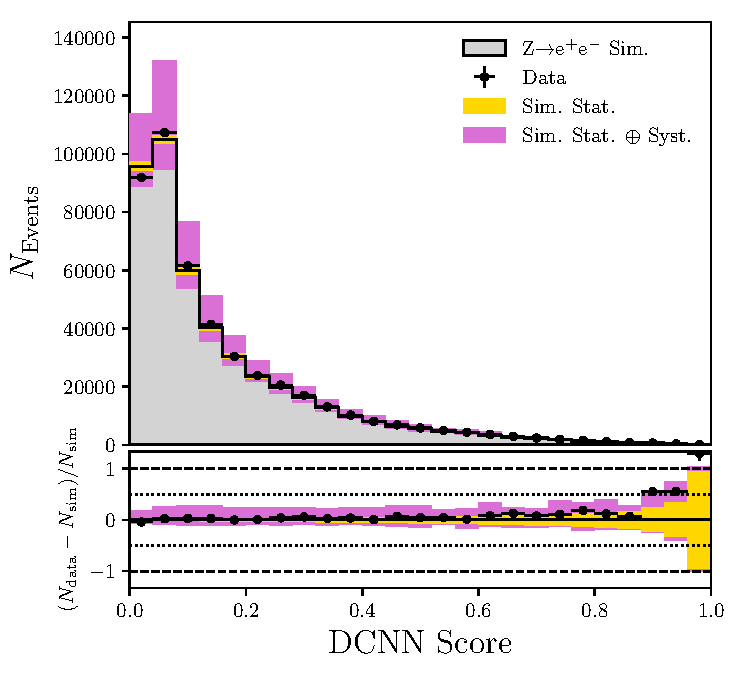
\includegraphics[width=0.49\textwidth]{figures/event_selection/int_score_zee_LPS.pdf}
    \end{center}
    \caption{\Zee validation plots for the output scores of the image-only network (left) and the full network (right).}
    \label{fig:event_categorisation:int_score_zee}
\end{figure}

Generally, the agreement is good with a very slight shift in the image-only model. This suggests that the real data is slightly more VBF-like. 
The systematics bands are slightly larger in the image-only model and at the lower end of the full DCNN score compared to the combined BDT. This difference may not be significant as it is located in a score region that is rejected by the DCNN VBF tag.  


To determine how the distribution of images differs between simulation and data, an images-only DCNN is trained to discriminate between them.
This network will have the same structure, regularisation, loss and training process as step one of the VBF DCNN model. 
Once trained the performance of this network is evaluated and the features it has built are analysed to learn about the image distribution disagreement.  
The performance of the data/simulation discriminant is shown in Figure \ref{fig:event_categorisation:zee_disc_perf}.
\begin{figure}[h!]
    \centering
    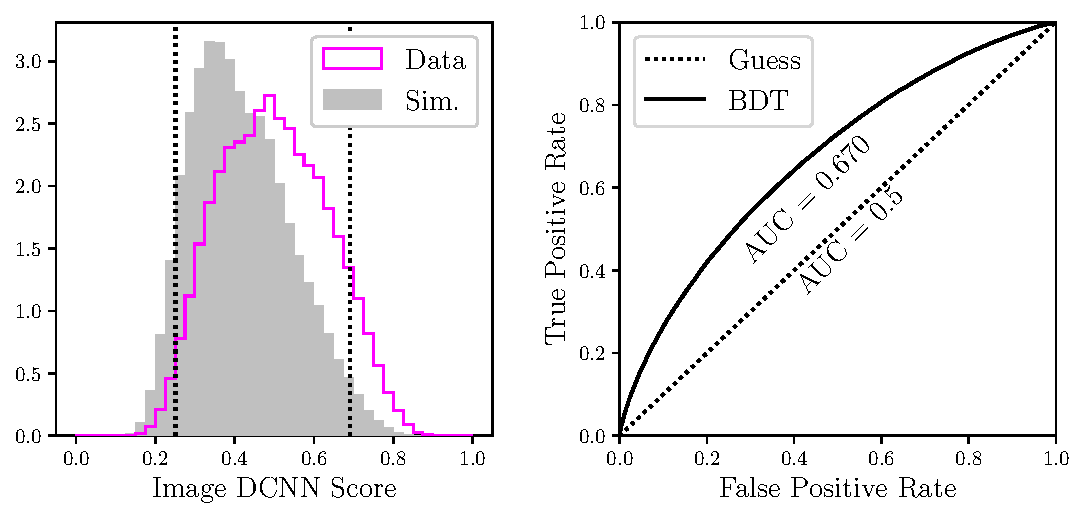
\includegraphics[width=0.8\textwidth]{figures/event_selection/ROC_Zee_img_DCNN.pdf}
    \caption{\Zee Simulation/data discriminant performance. The score distribution for the simulation and data classes is shown on the left, and the associated ROC curve is shown on the right.} 
    \label{fig:event_categorisation:zee_disc_perf}
\end{figure}

The AUROC suggests that there is indeed detectable disagreement in the image distributions. 
However, the network score validation's level of agreement suggests that although there is disagreement the network is fairly robust to it. 

To extract the areas of disagreement between the image datasets from the network the same interpretation techniques described previously are used. 
First feature visualisation is used to produce images that contain a collection of discriminating features (Figure \ref{fig:event_categorisation:zee_data_sim_feature_vis}).
\begin{figure}[h!]
    \begin{center}
        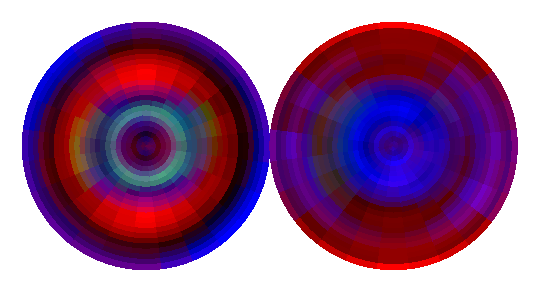
\includegraphics[width=0.85\textwidth]{figures/event_selection/zee_norm_logits0.pdf}
        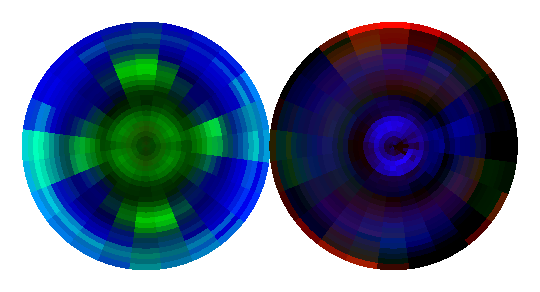
\includegraphics[width=0.85\textwidth]{figures/event_selection/zee_norm_logits1.pdf}
    \end{center}
    \caption{Sim/Data discriminant feature visualisation. The top dijet image is optimised for the simulation output neuron, and the bottom is optimised for the data neuron.} 
    \label{fig:event_categorisation:zee_data_sim_feature_vis}
\end{figure}

The difference is most pronounced in the leading jet where there is more charged \pt deposition in simulation and a different structure. The simulation is more rounded and ggH-like, the data has radial bands of neutral \pt along the $\Delta\eta$, $\Delta\phi$ axes and appears more VBF-like.   
The subleading jet appears to be similar in shape between the two classes but with more charged \pt in the simulation and a more collimated jet in data. Overall the data class visualisation has more VBF-like qualities and the simulation is more ggH-like. 

To verify the feature visualisation, maximally activating images are inspected for the most simulation-like and most data-like events according to the model (Figure \ref{fig:event_categorisation:zee_data_sim_max_act}. 
\begin{figure}[h!]
    \begin{center}
        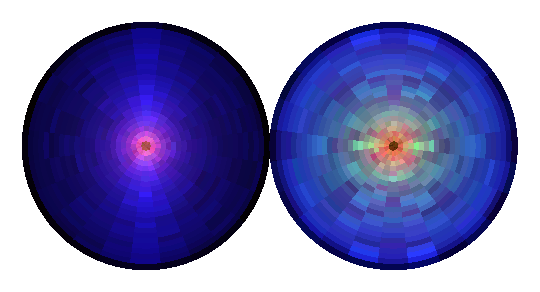
\includegraphics[width=0.85\textwidth]{figures/event_selection/zee_max_act_mean_sim.pdf}
        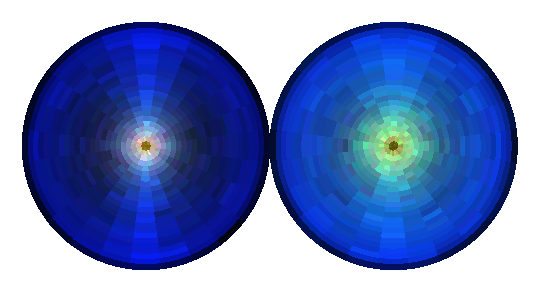
\includegraphics[width=0.85\textwidth]{figures/event_selection/zee_max_act_mean_data.pdf}
    \end{center}
    \caption{Mean images for top and bottom 5\% maximally activating events. 
             Score selection for simulation-like is shown at the top, selection for data-like is at the bottom.}
    \label{fig:event_categorisation:zee_data_sim_max_act}
\end{figure}

These selected samples have a class purity of approximately 85\%, and they resemble the generated images. The image feature differences extracted with feature visualisation appear to be physically sensible. 
The difference in charged-\pt deposition is especially pronounced in these images, but a few other features are apparent. In the leading jet data-like sample there is a spread along the $\Delta\phi$ axis that is much less pronounced in the simulation-like sample. 
The smooth appearance of the neutral-\pt channel in the data-like subleading jet also suggests that there is more neutral deposition within the tracker acceptance. 



\subsubsection{QCD Modelling Variations}
The model is evaluated over samples that explicitly differ in their modelling of QCD with the same procedure as the BDT-based model.
These consist of up and down variations that should encompass the behaviour of real data.
The resulting score distribution variation and the variations in the ROC curves for both image-only and the full model are shown in Figure \ref{fig:event_categorisation:DCNN_psvar}.
\begin{figure}[h!]
    \centering
    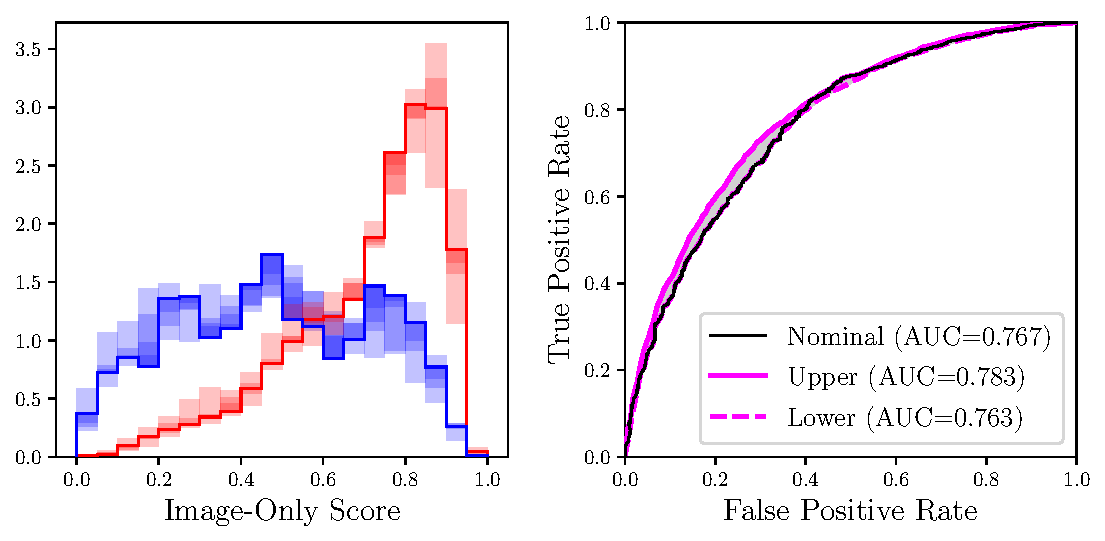
\includegraphics[width=0.80\textwidth]{figures/event_selection/imgonly_PSvar_PS.pdf}
    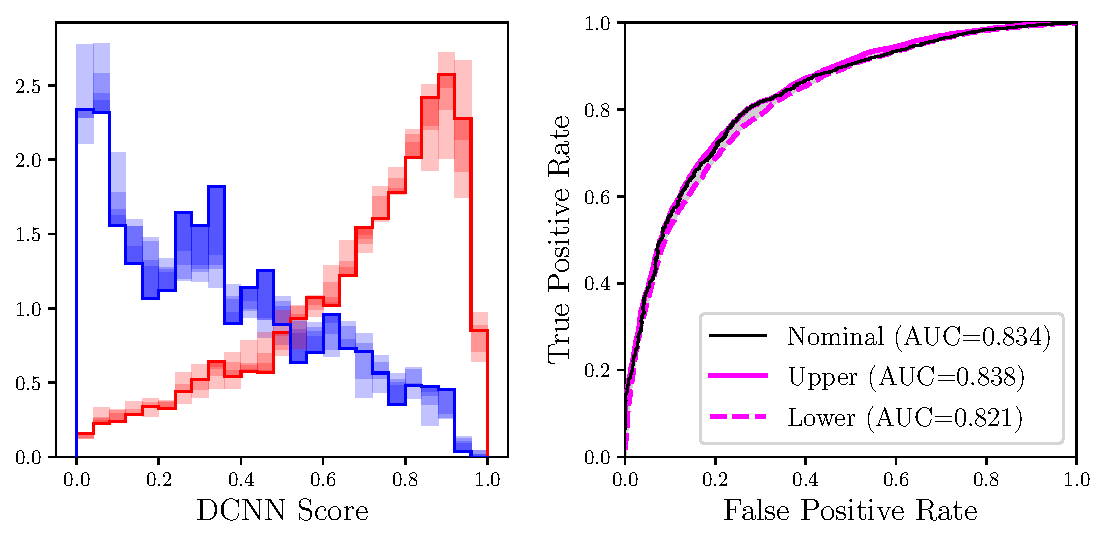
\includegraphics[width=0.80\textwidth]{figures/event_selection/int_PSvar_PS.pdf}
    \caption{Variation in the score distributions and ROC curves with parton shower and underlying event variation. The top pair corresponds to the image-only model (step 1 of training) and the bottom plots correspond to the full model used in the tag.}
    \label{fig:event_categorisation:DCNN_psvar}
\end{figure}

Remarkably, the image-only model is not only robust to these variations but actually has a higher AUROC and therefore better performance on the QCD variation samples.
This robustness suggests that the learned features are physically well-motivated as the features found in data should be within these variations.
The full model shows a small degradation in discrimination power, but at a level comparable to the combined BDT. 

\subsection{Conclusions}
Dijet images have been demonstrated to encode useful discriminating features and that a dense CNN is capable of extracting them. These features are found to be robust to QCD modelling variations, and the overall response of the model is similar between simulation and data. 

For model development Bayesian optimisation is a powerful technique for navigating possible hyperparameter choices. The final model is a powerful discriminant, but compromises must be made due to the relationship between VBF/ggH discrimination and overall signal significance. 
To approach this tradeoff correctly and to tune for the right choice the notion of cost sensitivity needs to be introduced during training. This is the correct way to set the priority between these two aspects of VBF tag model performance. 

The main impact on tag performance is reducing ggH contamination. This sort of technique will be more useful for targeting high-purity samples of particular processes rather than enhanced signal significance. 

Finally, the common criticism that CNNs are black boxes is shown not to be the case. There are many techniques available to interpret them and only a few are used here. Feature visualisation and max-activation images can be used to look inside the network at single neurons, feature maps or even entire feature volumes to determine what they are looking for. 
Furthermore the above techniques can be used to analyse data/simulation compatibility and isolate features from regions of disagreement. 



